\documentclass[a4paper,12pt]{article}
\usepackage[utf8]{inputenc}
\usepackage[T1]{fontenc}
\usepackage{geometry}
\geometry{margin=1in}
\usepackage{graphicx}
\usepackage{caption}
\usepackage{hyperref}
\usepackage{amsmath}
\usepackage{booktabs}

% Preamble for document structure
\title{OPL Website CI/CD Case Study}
\author{Hushng Fikrat Muhibullah, Anju, Kaif, Muskaan}
\date{August 05, 2025}

\begin{document}

\maketitle

\section{Introduction}
This case study documents the comprehensive implementation of a Continuous Integration/Continuous Deployment (CI/CD) pipeline for the Oshawa Public Library (OPL) website using Amazon Web Services (AWS) Elastic Container Service (ECS). The project was executed by a team comprising Hushng Fikrat Muhibullah, Anju, Kaif, and Muskaan, with each member contributing specialized skills. This document incorporates screenshots as proof of implementation, detailing network configuration, security setups, task definitions, workflows, IAM roles, service deployment, troubleshooting, and architectural diagrams.

\section{Team Responsibilities}
\begin{itemize}
    \item \textbf{Hushng Fikrat Muhibullah (Team Leader)}: Managed and assigned tasks, handled Docker installation and containerization, collaborated with Kaif on security design and CI/CD workflow draft, worked with Anju on architectural diagram and CI/CD documentation completion, led final document compilation and review, oversaw presentation rehearsal and finalization, and supervised document and presentation submission.
    \item \textbf{Kaif}: Created ECS and ECR resources, collaborated with Hushng on security design and CI/CD workflow draft.
    \item \textbf{Muskaan}: Configured network settings (VPC, Subnet, Internet Gateway, Security Groups), collaborated with Anju on the initial architecture draft, and participated in presentation rehearsal and finalization.
    \item \textbf{Anju}: Prepared all documentation and presentation materials, collaborated with Muskaan on the initial architecture draft, worked with Hushng on architectural diagram and CI/CD documentation completion, drafted the presentation slide deck, contributed to final document compilation and review, and participated in presentation rehearsal and finalization.
\end{itemize}

\section{Implementation Steps}

\subsection{Local Setup and Dockerization}
\begin{figure}[h]
    \centering
    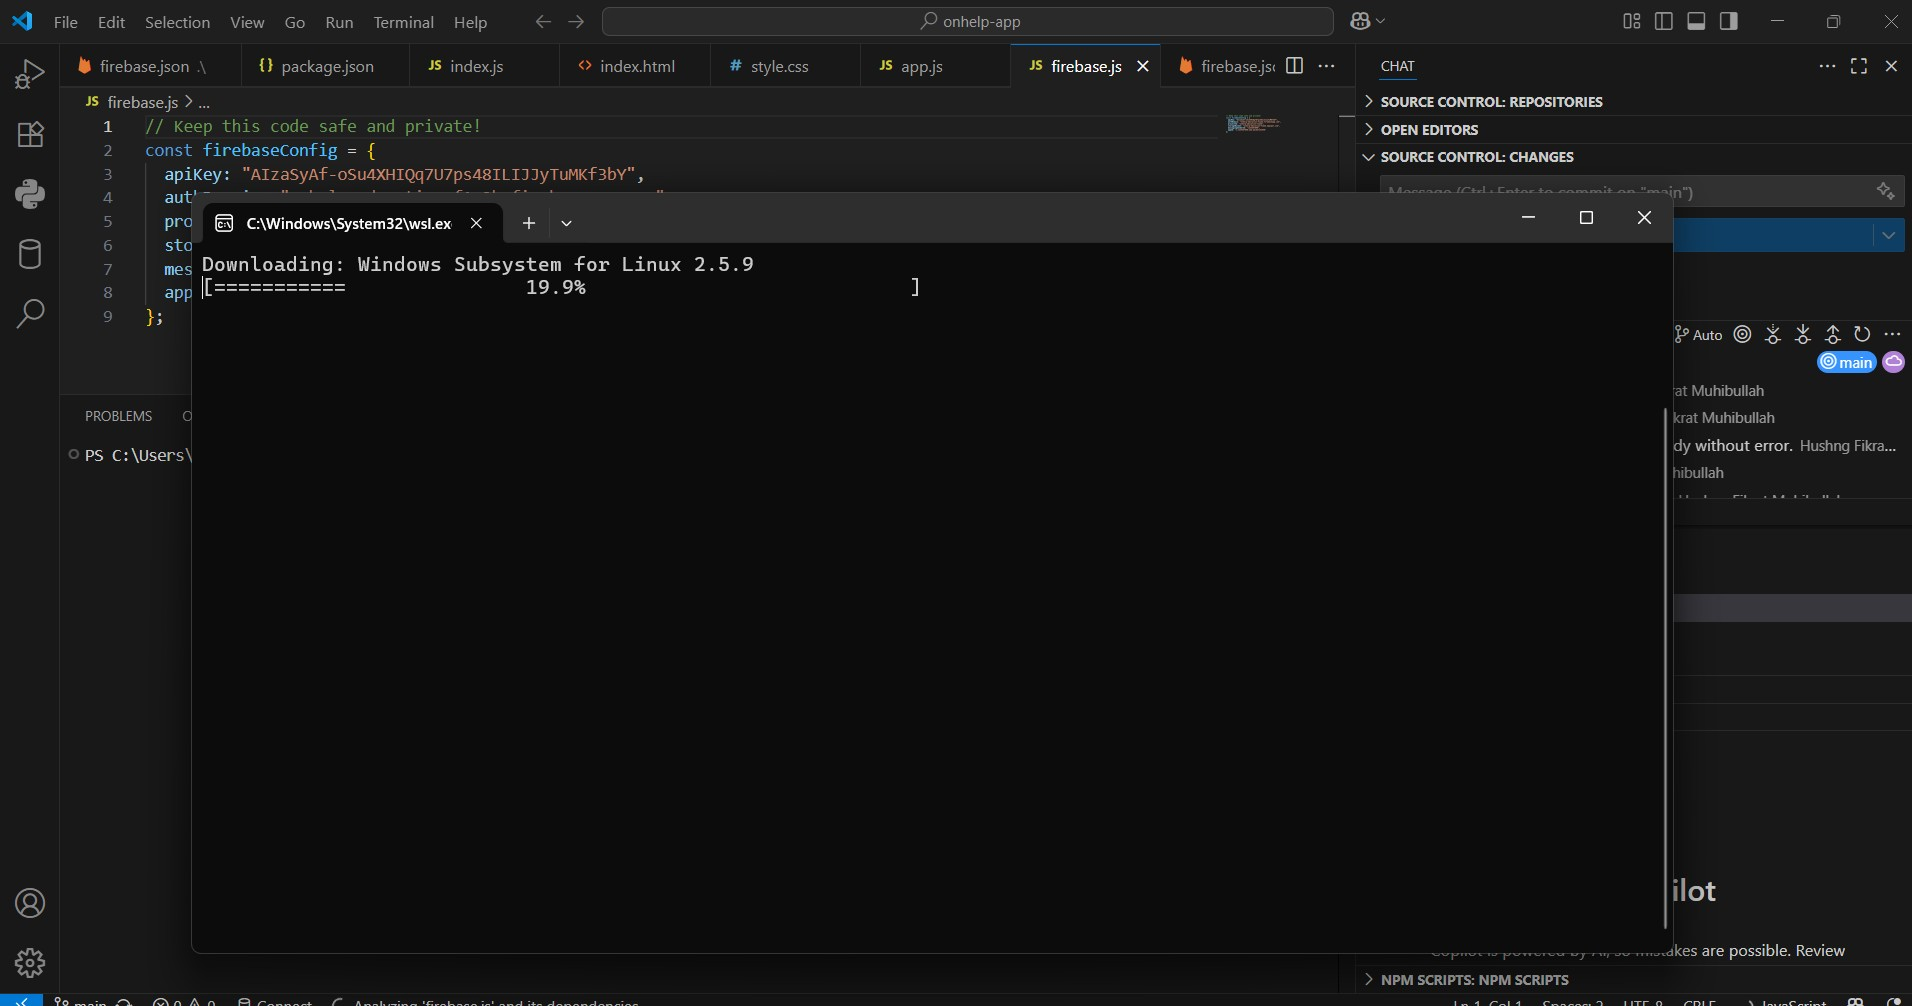
\includegraphics[width=0.8\textwidth]{WSL installation.jpg}
    \caption{WSL installation, a prerequisite for Docker on Windows.}
\end{figure}
\begin{figure}[h]
    \centering
    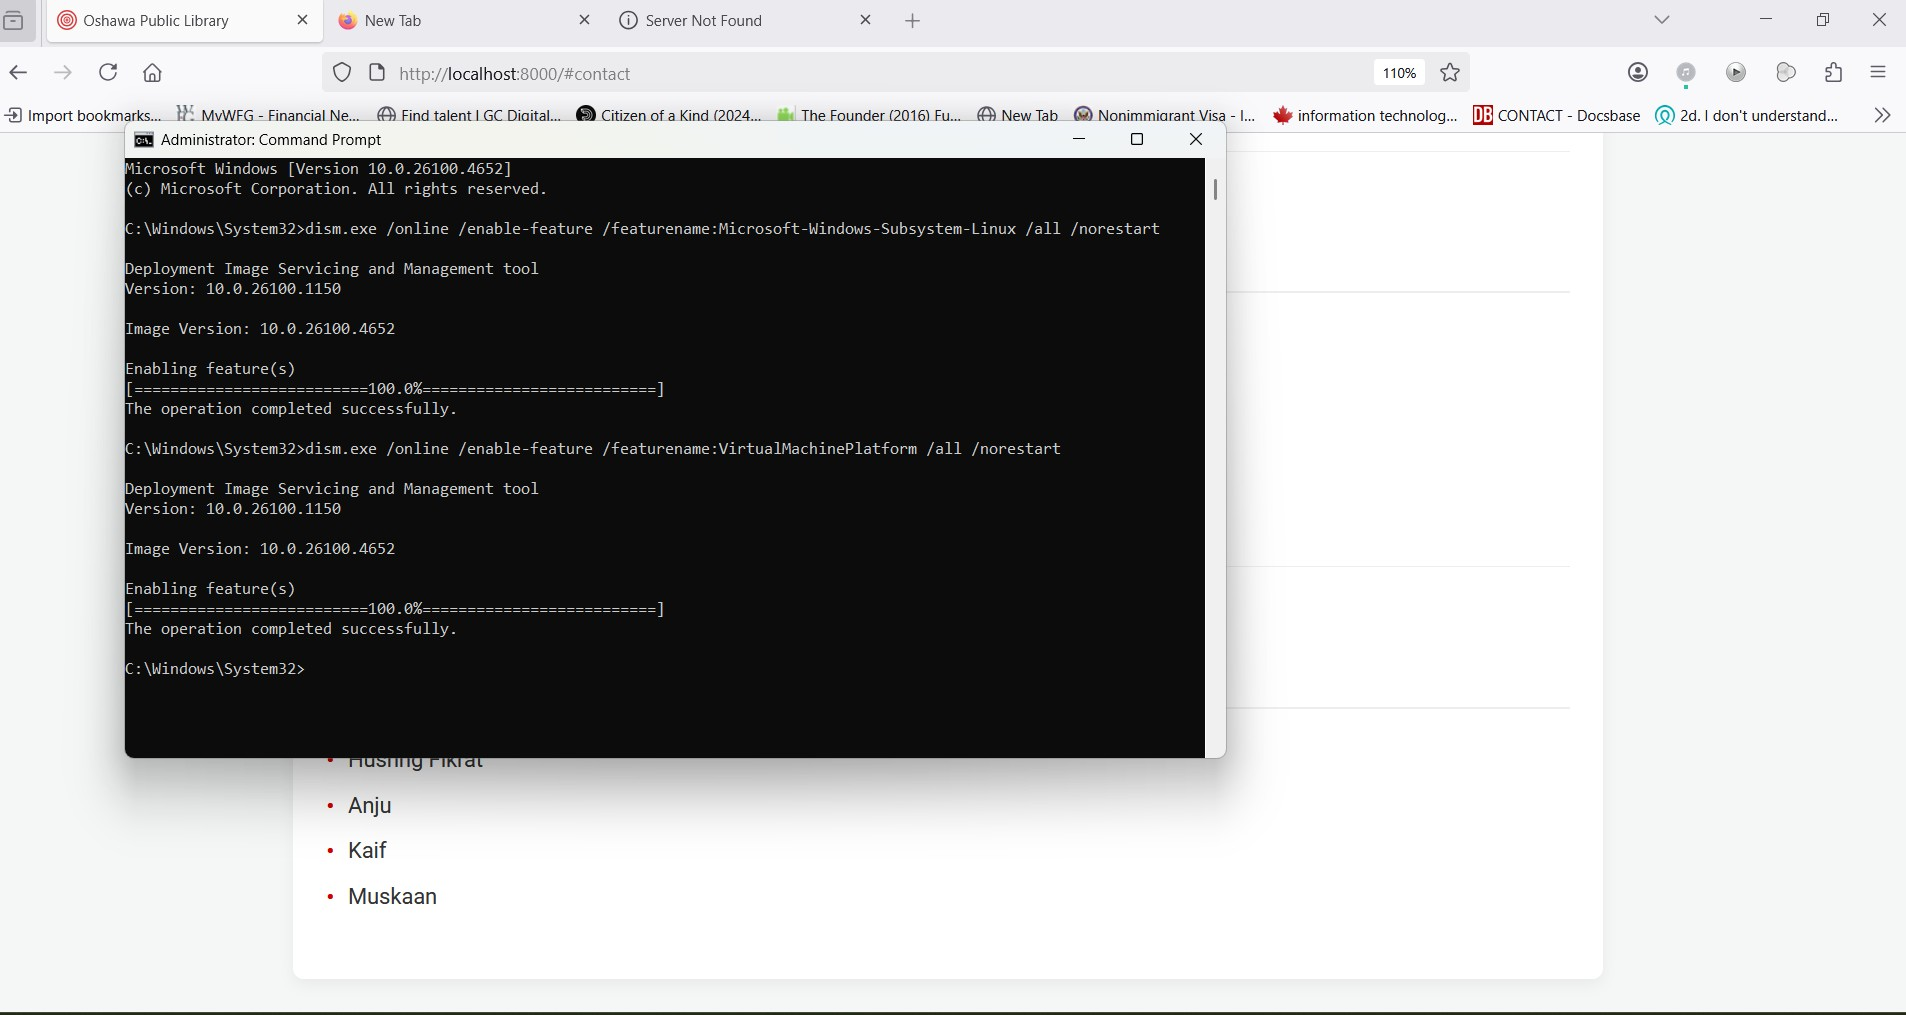
\includegraphics[width=0.8\textwidth]{Docker_installation_requirement_package.jpg}
    \caption{Installation of required packages for Docker setup.}
\end{figure}
\begin{figure}[h]
    \centering
    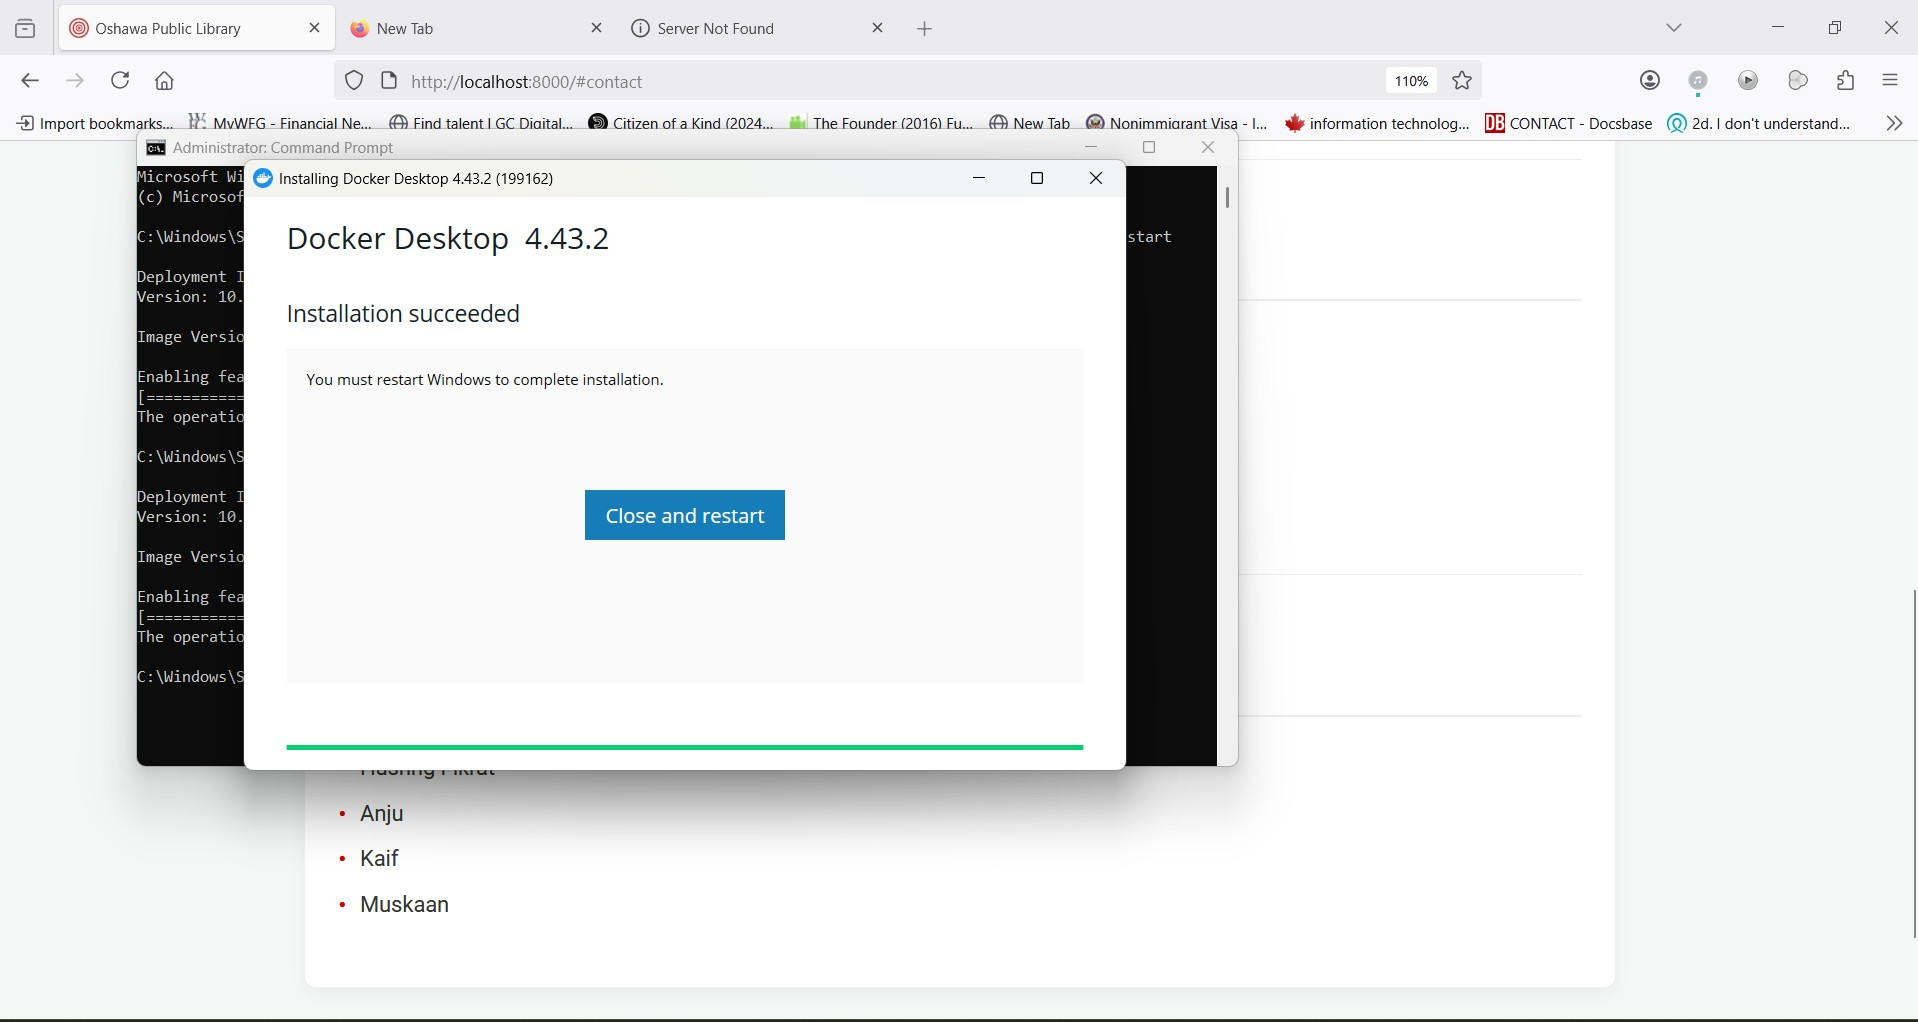
\includegraphics[width=0.8\textwidth]{Docker_installation.jpg}
    \caption{Successful completion of Docker installation.}
\end{figure}
\begin{figure}[h]
    \centering
    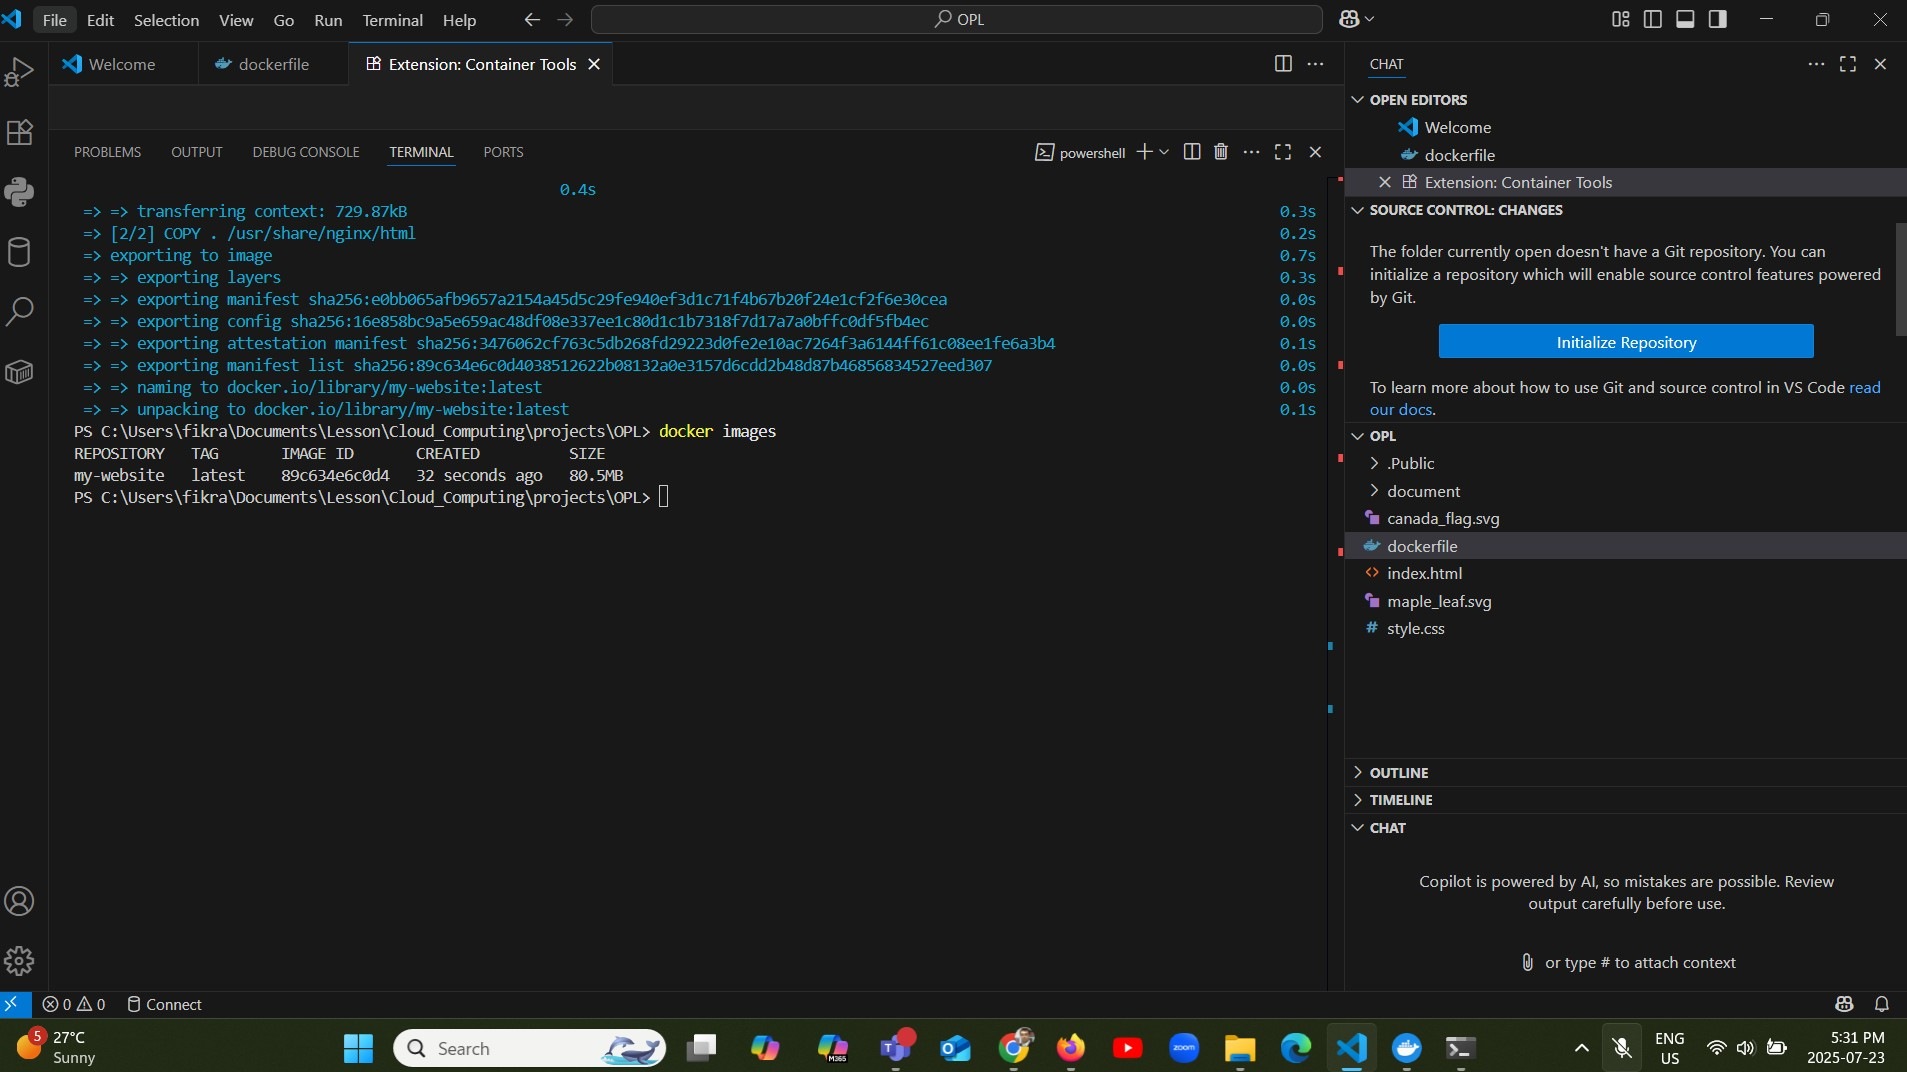
\includegraphics[width=0.8\textwidth]{docker_image_created.jpg}
    \caption{The Docker image for the web application is successfully created.}
\end{figure}
\begin{figure}[h]
    \centering
    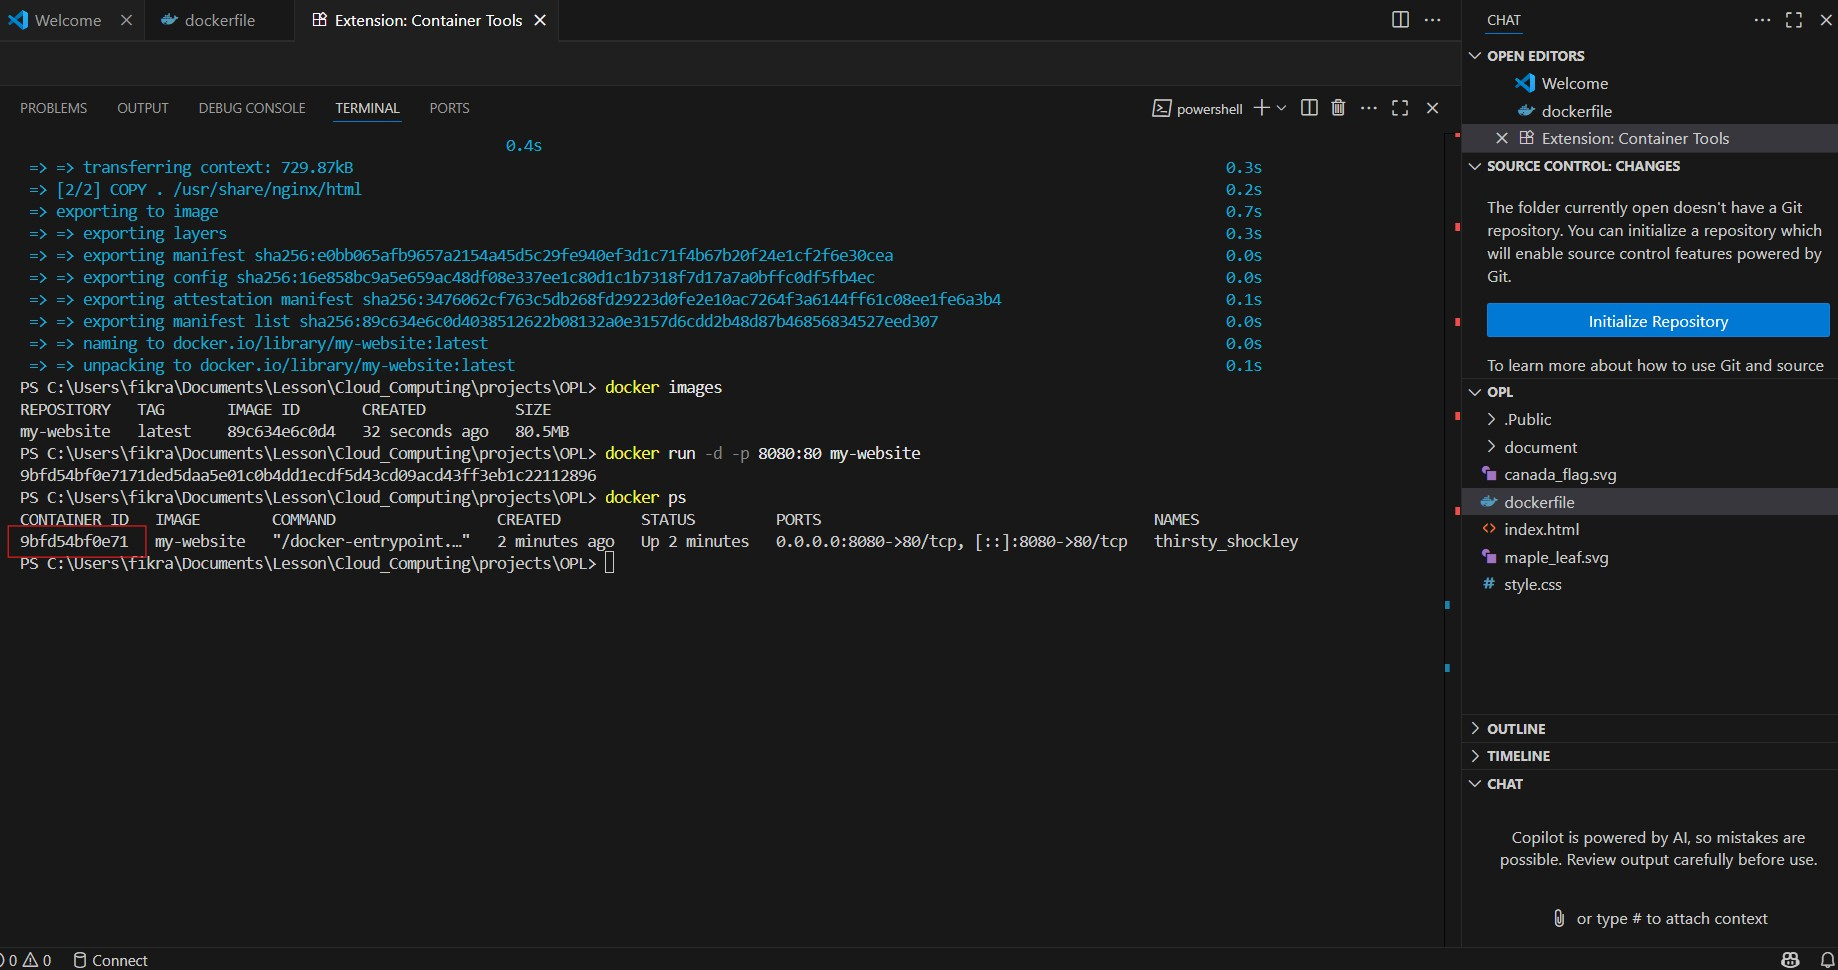
\includegraphics[width=0.8\textwidth]{docker_containerID.jpg}
    \caption{The Docker container running with its ID.}
\end{figure}
\begin{figure}[h]
    \centering
    
\includegraphics[width=0.8\textwidth]{webapp_running_via_docker.jpg}
    \caption{Verification that the web application is running locally via Docker on port 8080.}
\end{figure}
\begin{figure}[h]
    \centering
    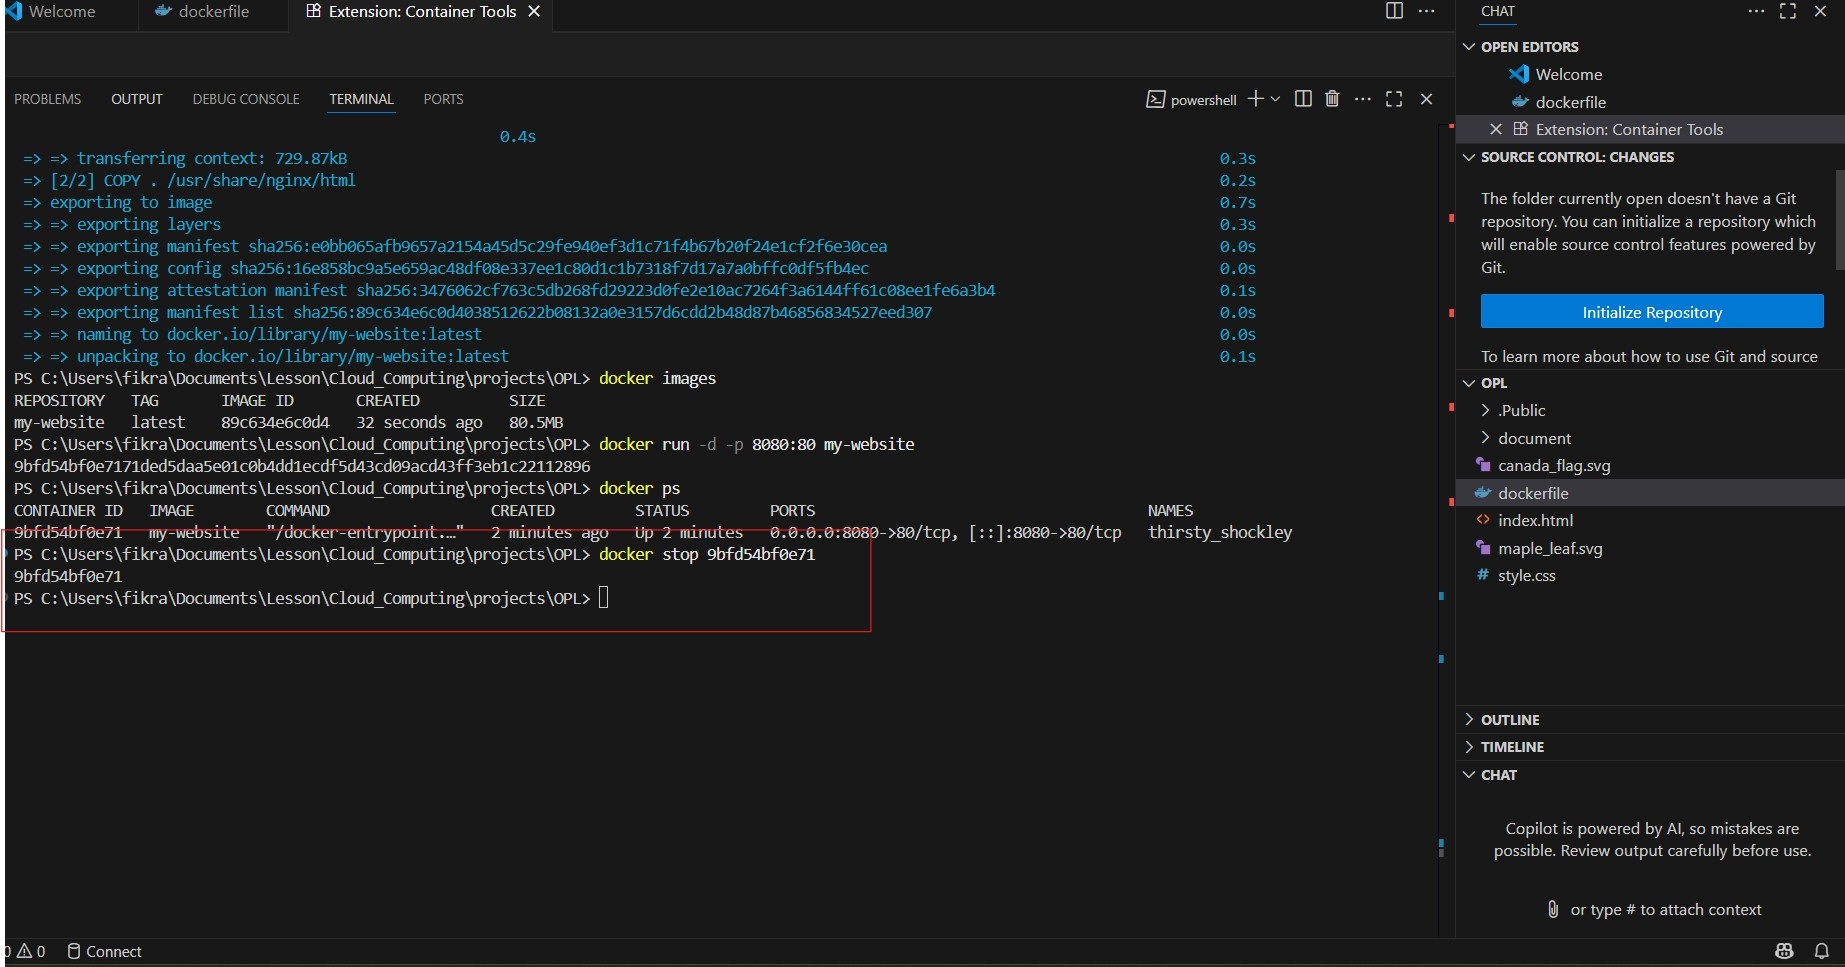
\includegraphics[width=0.8\textwidth]{local_docker_stopped.jpg}
    \caption{The local Docker container is stopped before deployment to AWS.}
\end{figure}

\subsection{AWS CLI and ECR Configuration}
\begin{figure}[h]
    \centering
    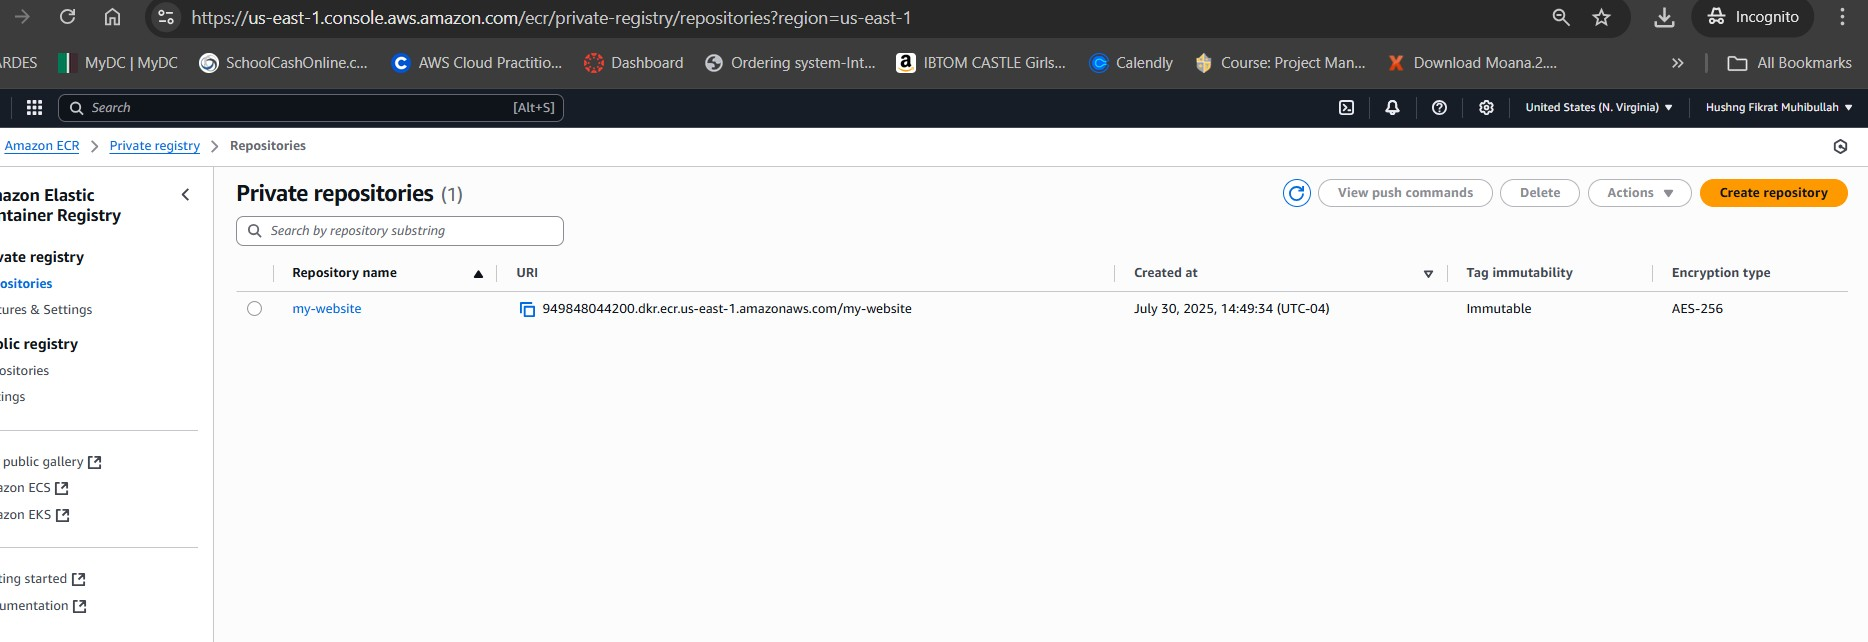
\includegraphics[width=0.8\textwidth]{ecr_repository_created.jpg}
    \caption{Creation of the ECR repository for storing the Docker image.}
\end{figure}
\begin{figure}[h]
    \centering
    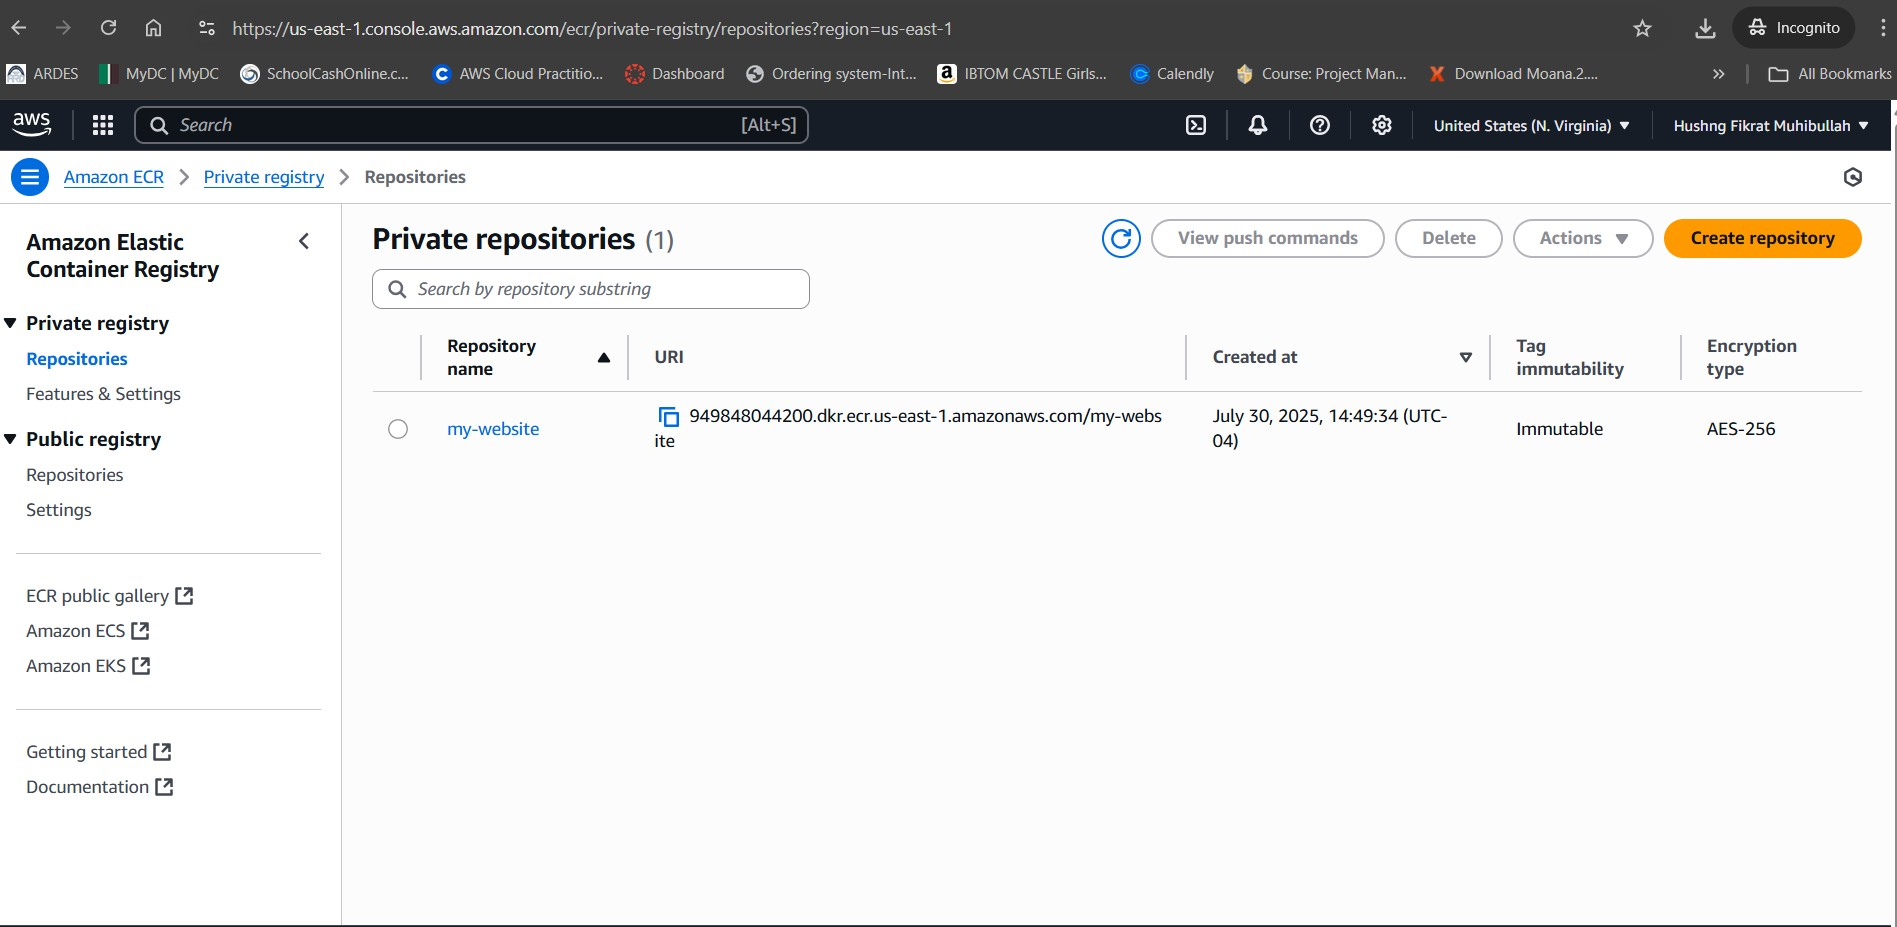
\includegraphics[width=0.8\textwidth]{ecr_1.jpg}
    \caption{Overview of the created ECR repository.}
\end{figure>
\begin{figure}[h]
    \centering
    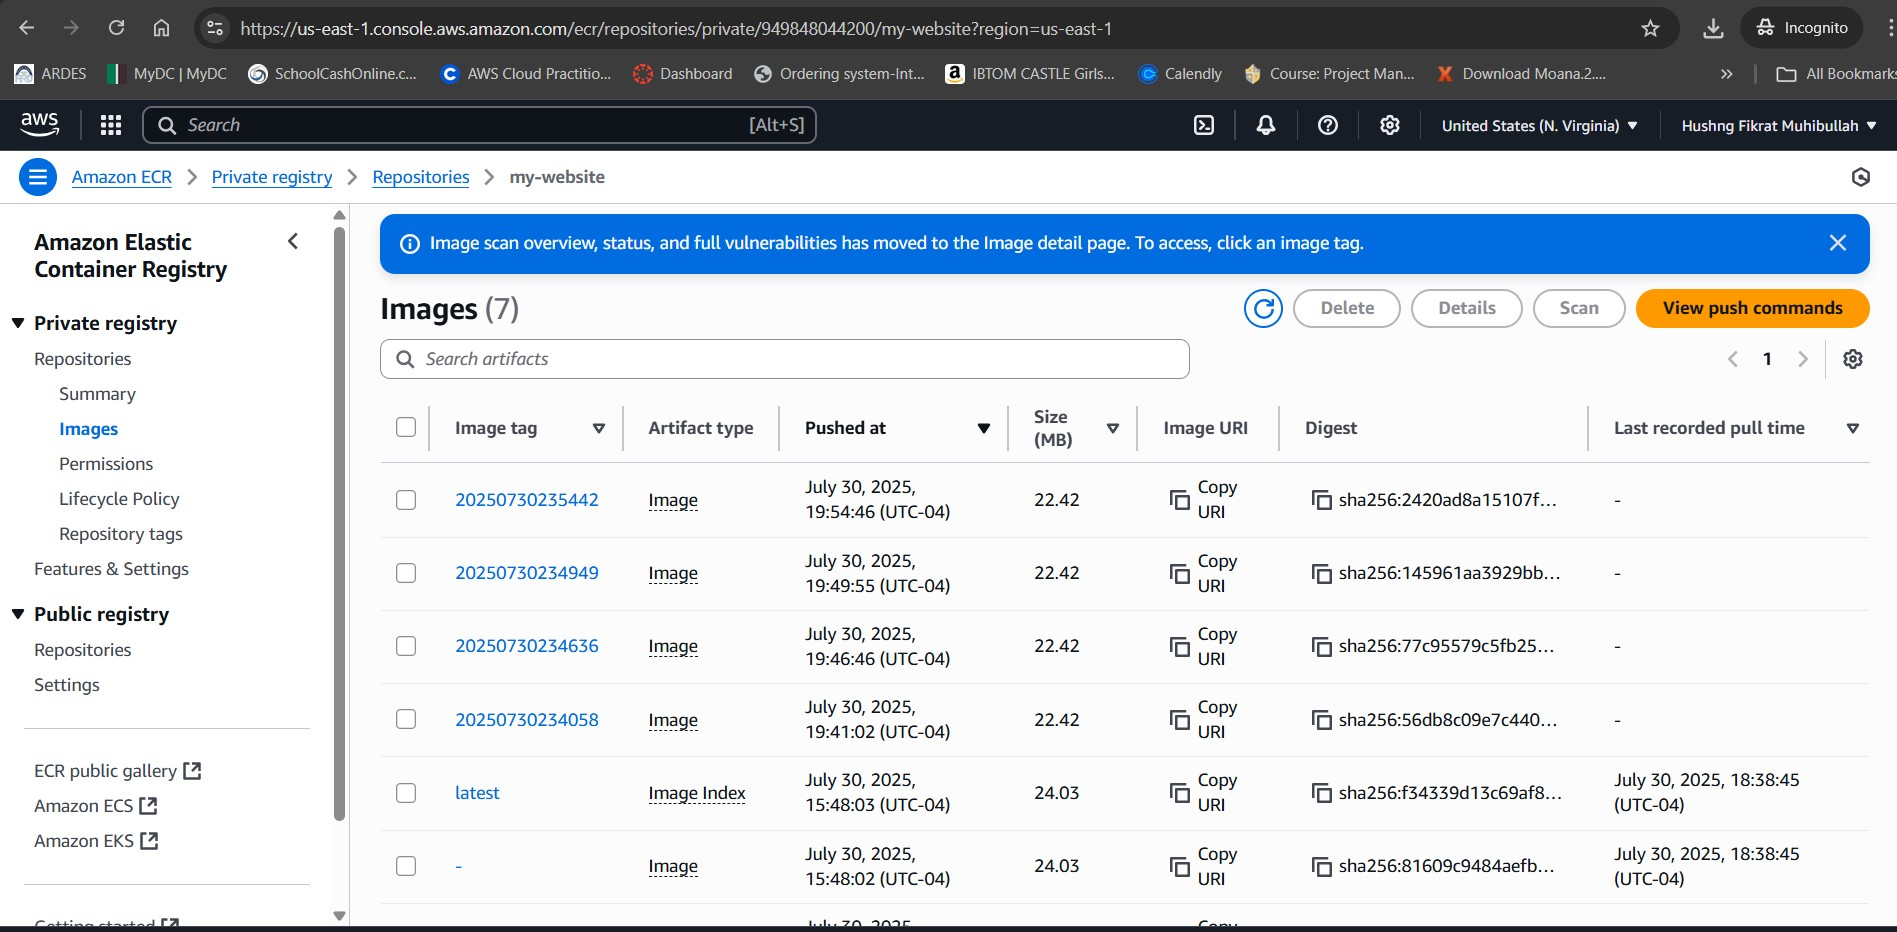
\includegraphics[width=0.8\textwidth]{ecr_2.jpg}
    \caption{The ECR repository is empty and ready for the image push.}
\end{figure>
\begin{figure}[h]
    \centering
    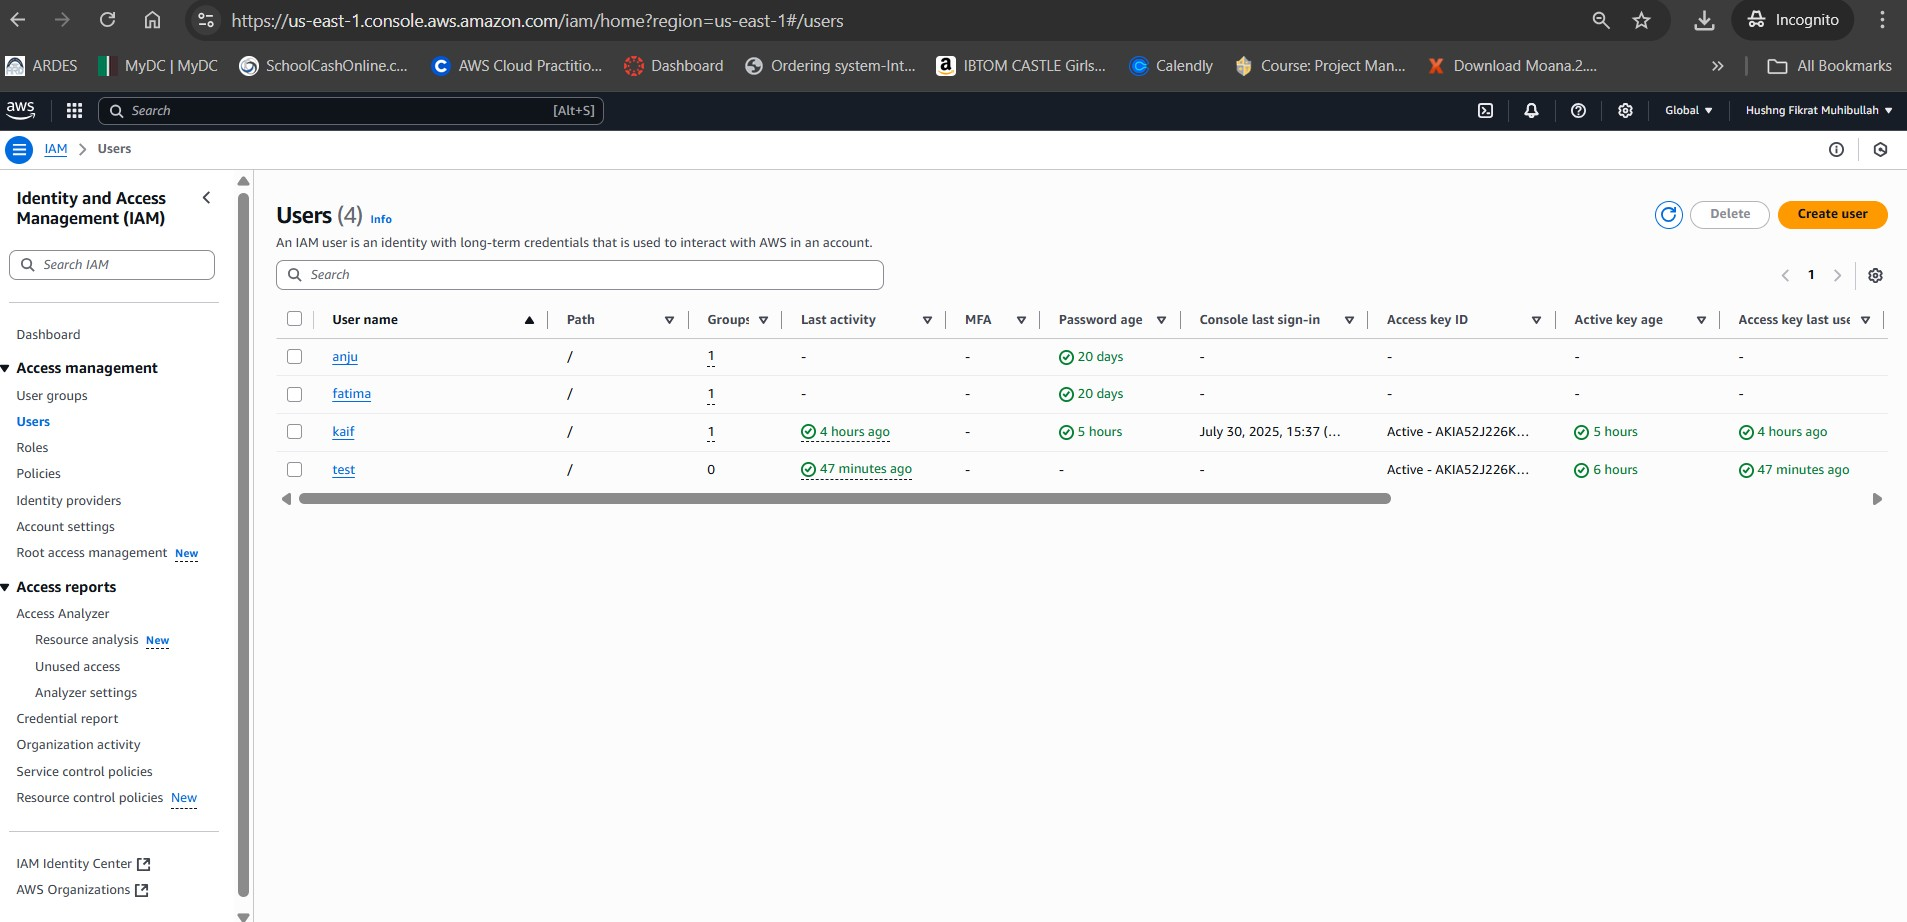
\includegraphics[width=0.8\textwidth]{User.jpg}
    \caption{User creation and IAM policy assignment.}
\end{figure}
\begin{figure}[h]
    \centering
    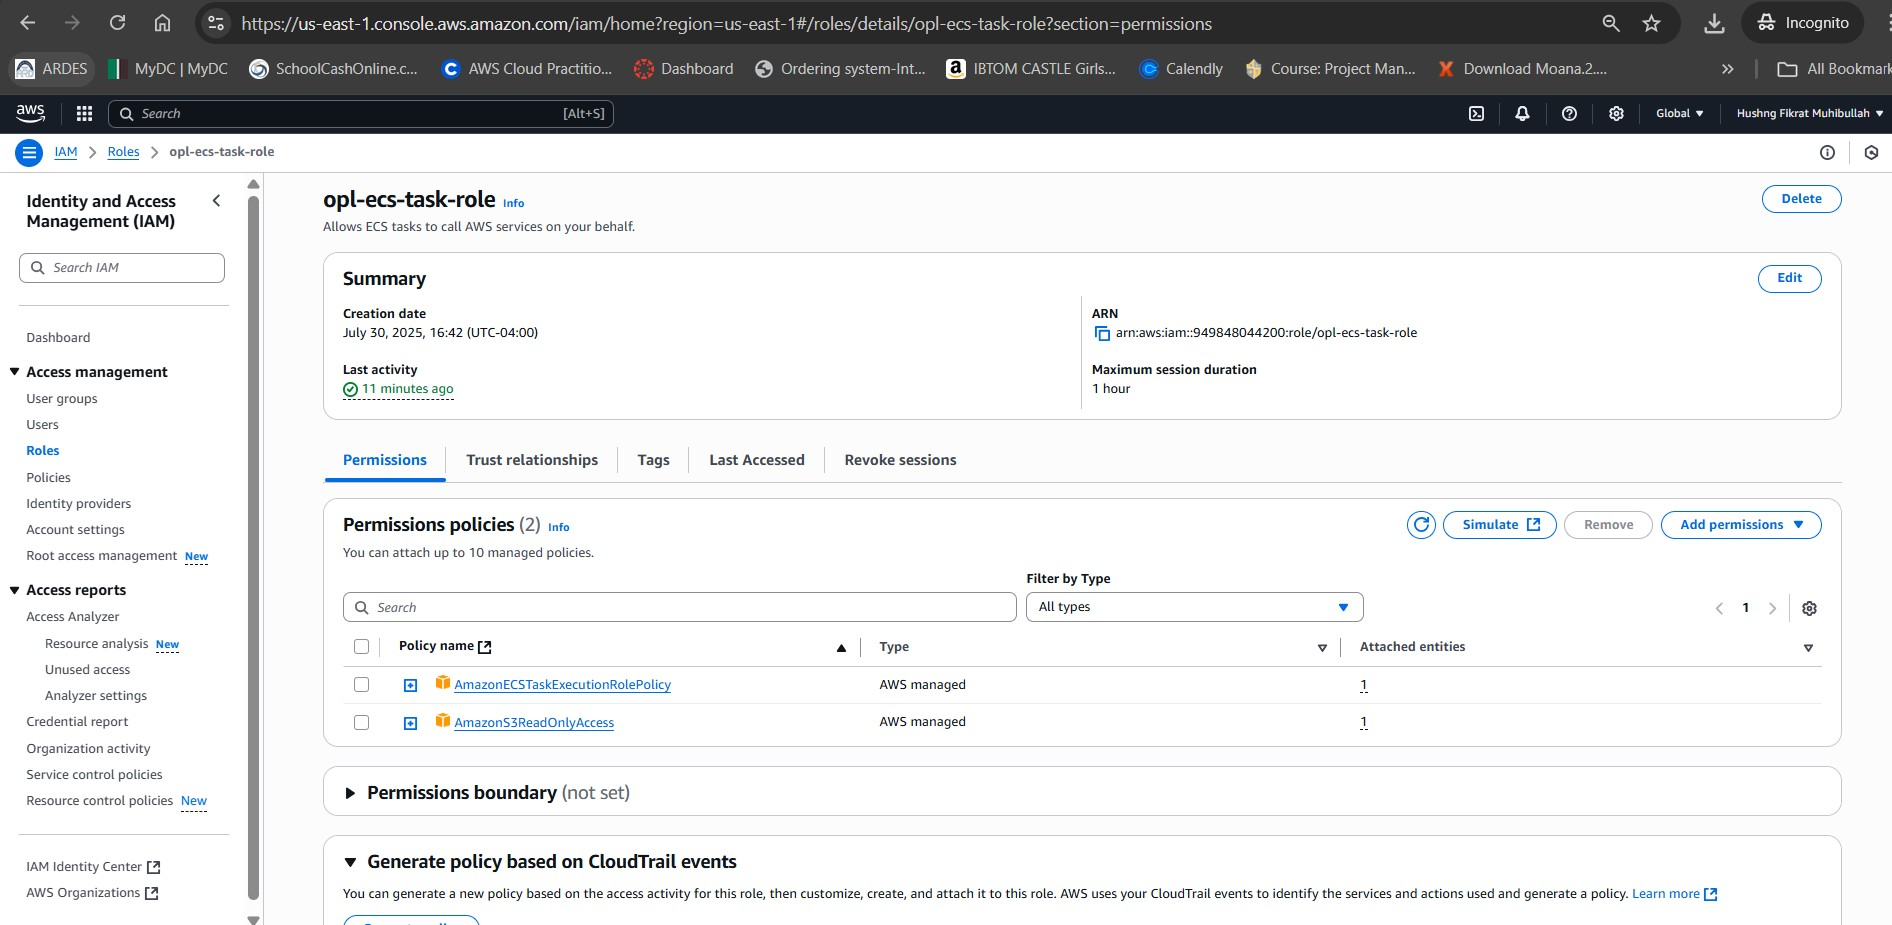
\includegraphics[width=0.8\textwidth]{Role.jpg}
    \caption{The IAM role creation with policies for ECS tasks.}
\end{figure}
\begin{figure}[h]
    \centering
    \includegraphics[width=0.8\textwidth]{aws_tools_installed.jpg}
    \caption{Installation of AWS Tools for PowerShell.}
\end{figure}
\begin{figure}[h]
    \centering
    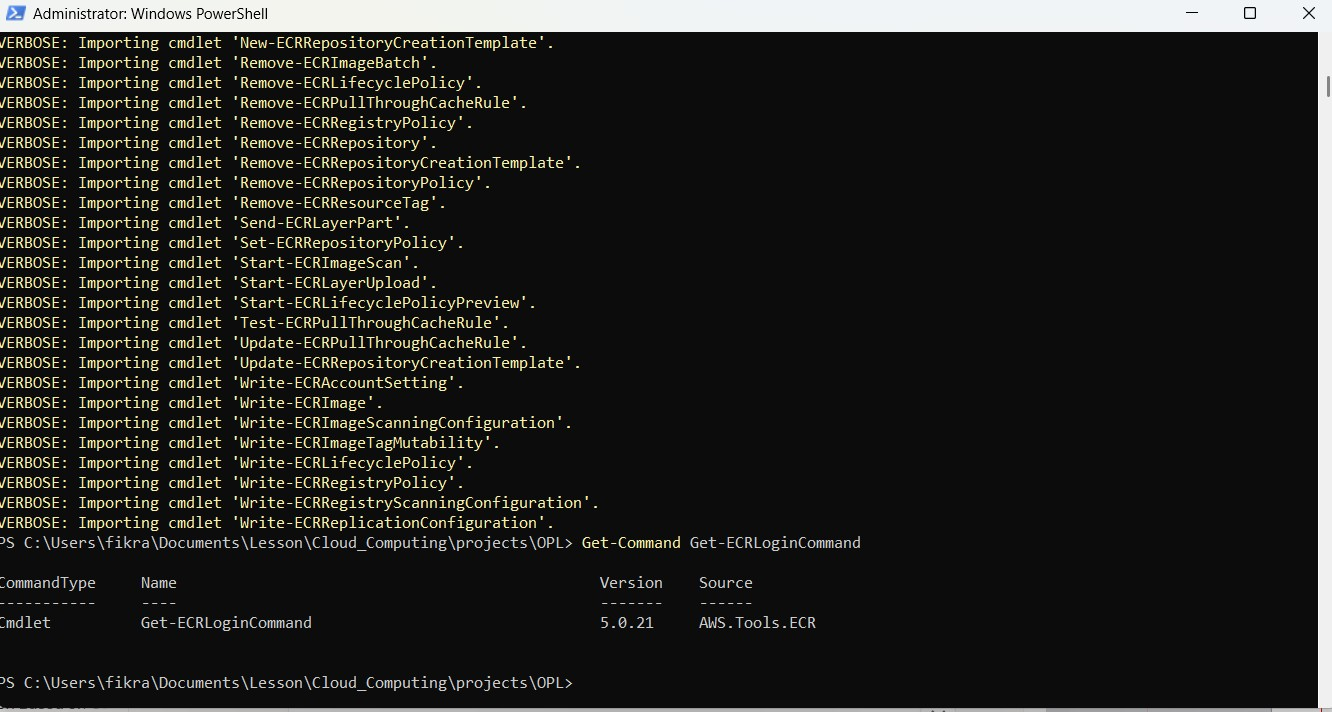
\includegraphics[width=0.8\textwidth]{AWS_tools_ECR installed.jpg}
    \caption{Verification that AWS Tools.ECR is installed.}
\end{figure>
\begin{figure}[h]
    \centering
    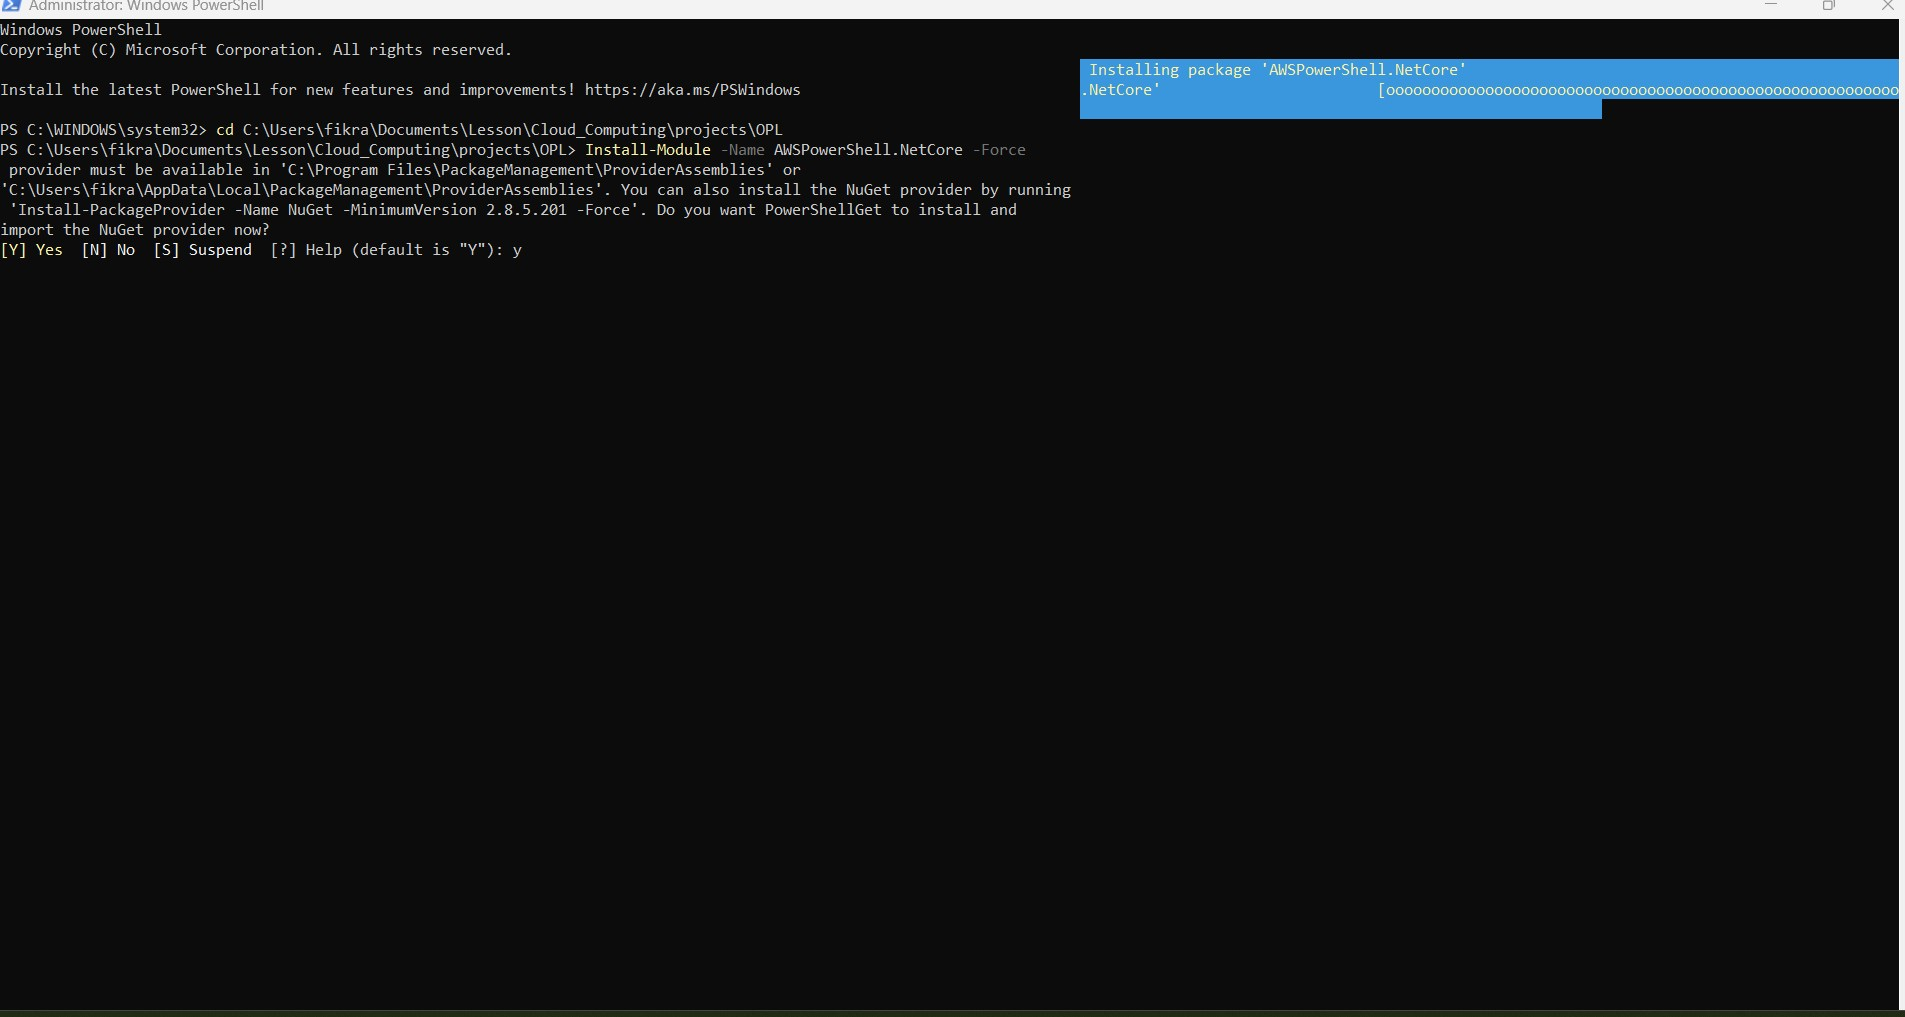
\includegraphics[width=0.8\textwidth]{AWS Tools for push commands-ECR.jpg}
    \caption{Push commands from ECR to upload the Docker image.}
\end{figure}
\begin{figure}[h]
    \centering
    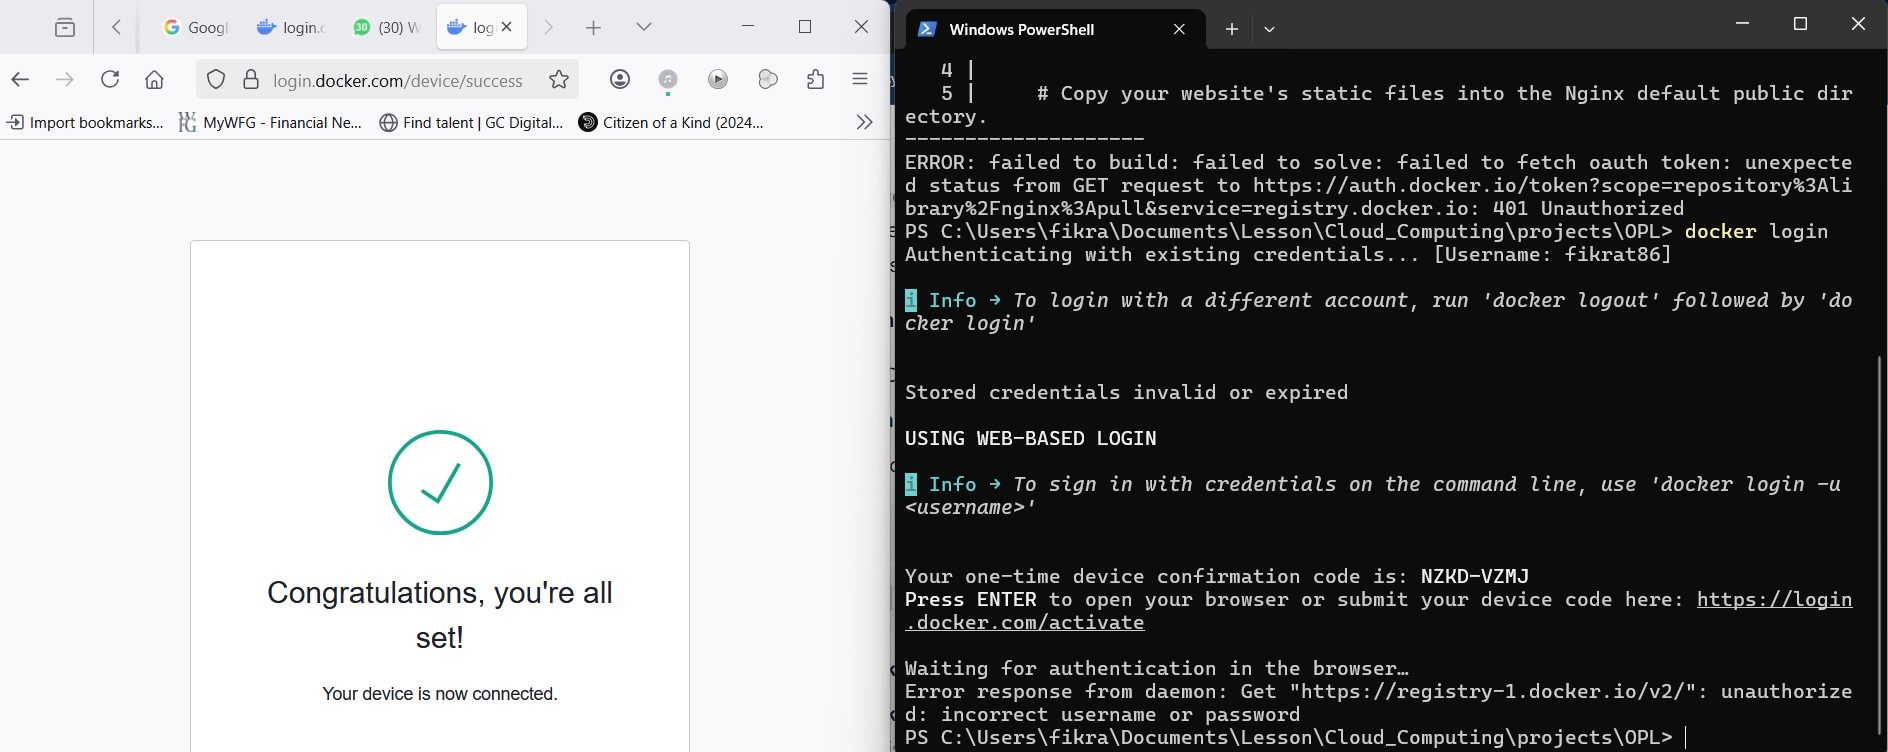
\includegraphics[width=0.8\textwidth]{login to docker.jpg}
    \caption{Docker login to ECR using the provided commands.}
\end{figure>
\begin{figure}[h]
    \centering
    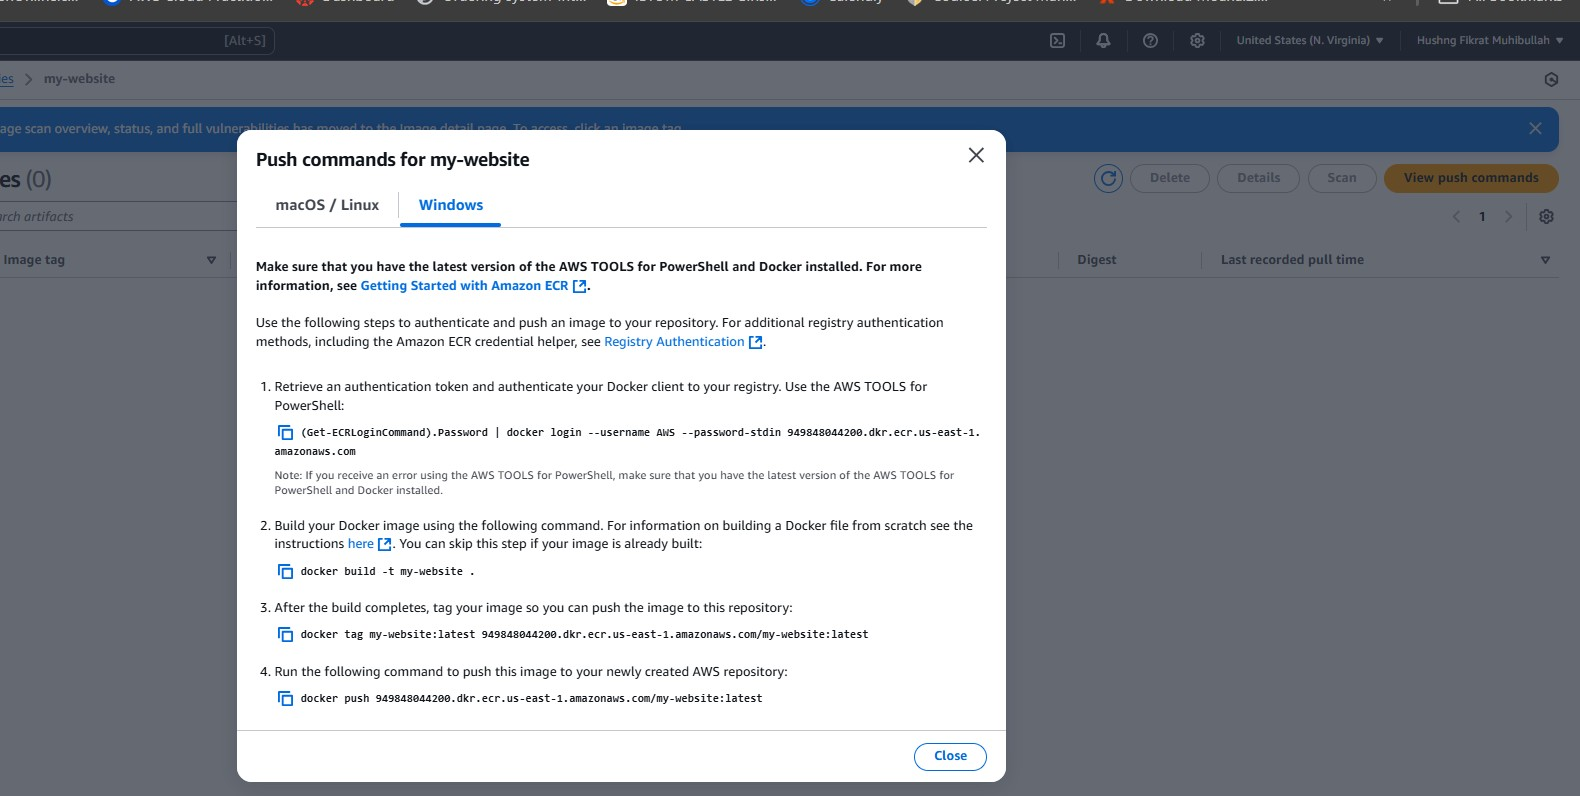
\includegraphics[width=0.8\textwidth]{ECR push command for my-website.jpg}
    \caption{The ECR push command for the `my-website` image.}
\end{figure>
\begin{figure}[h]
    \centering
    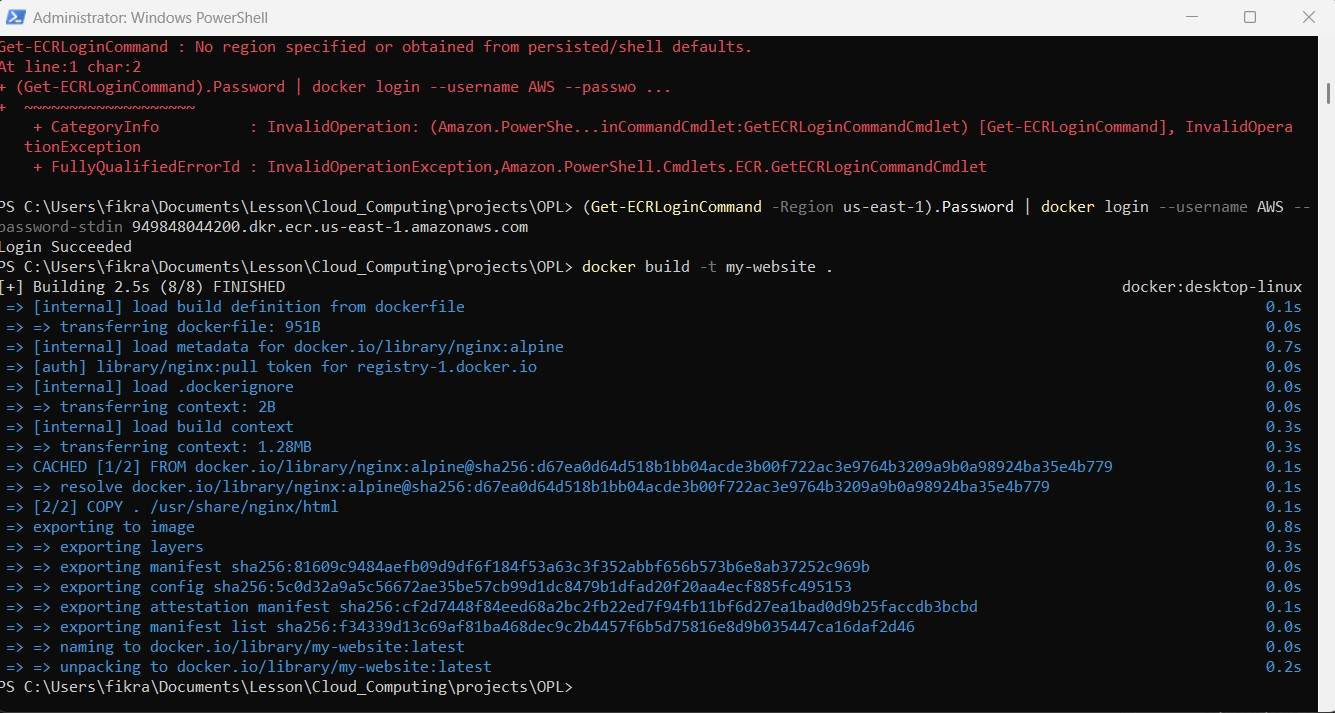
\includegraphics[width=0.8\textwidth]{push command-2 Export to ECR.jpg}
    \caption{Exporting the Docker image before pushing to ECR.}
\end{figure>
\begin{figure}[h]
    \centering
    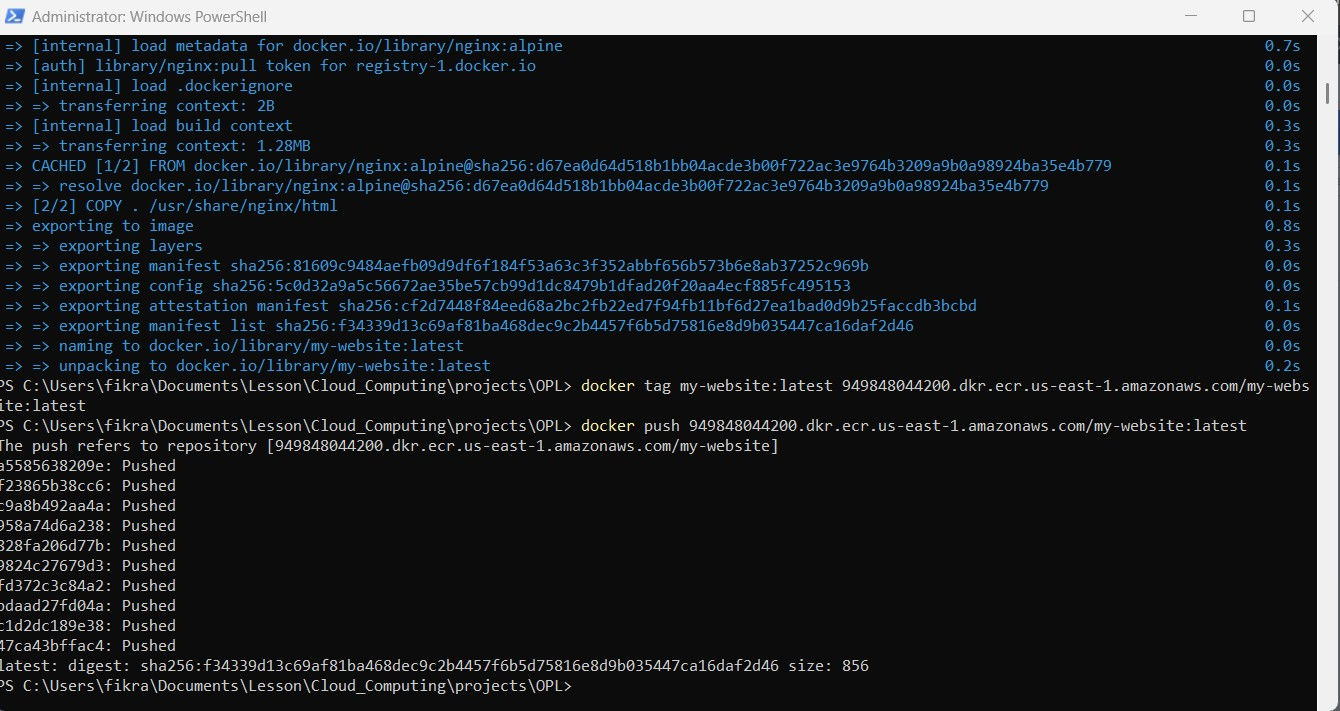
\includegraphics[width=0.8\textwidth]{push command-step3-4-5.jpg}
    \caption{Steps to tag and push the Docker image to ECR.}
\end{figure>
\begin{figure}[h]
    \centering
    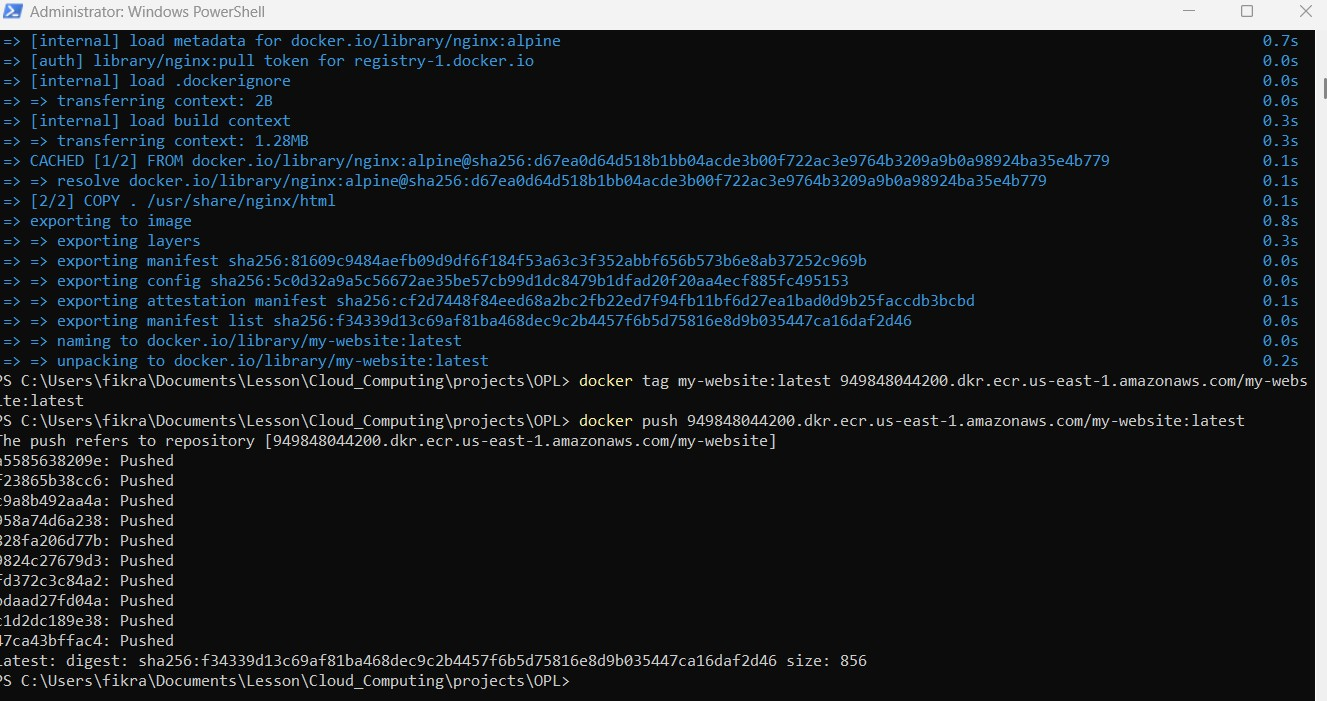
\includegraphics[width=0.8\textwidth]{push docker.jpg}
    \caption{The Docker image is successfully pushed to ECR.}
\end{figure>

\subsection{VPC and Subnet Configuration}
\begin{figure}[h]
    \centering
    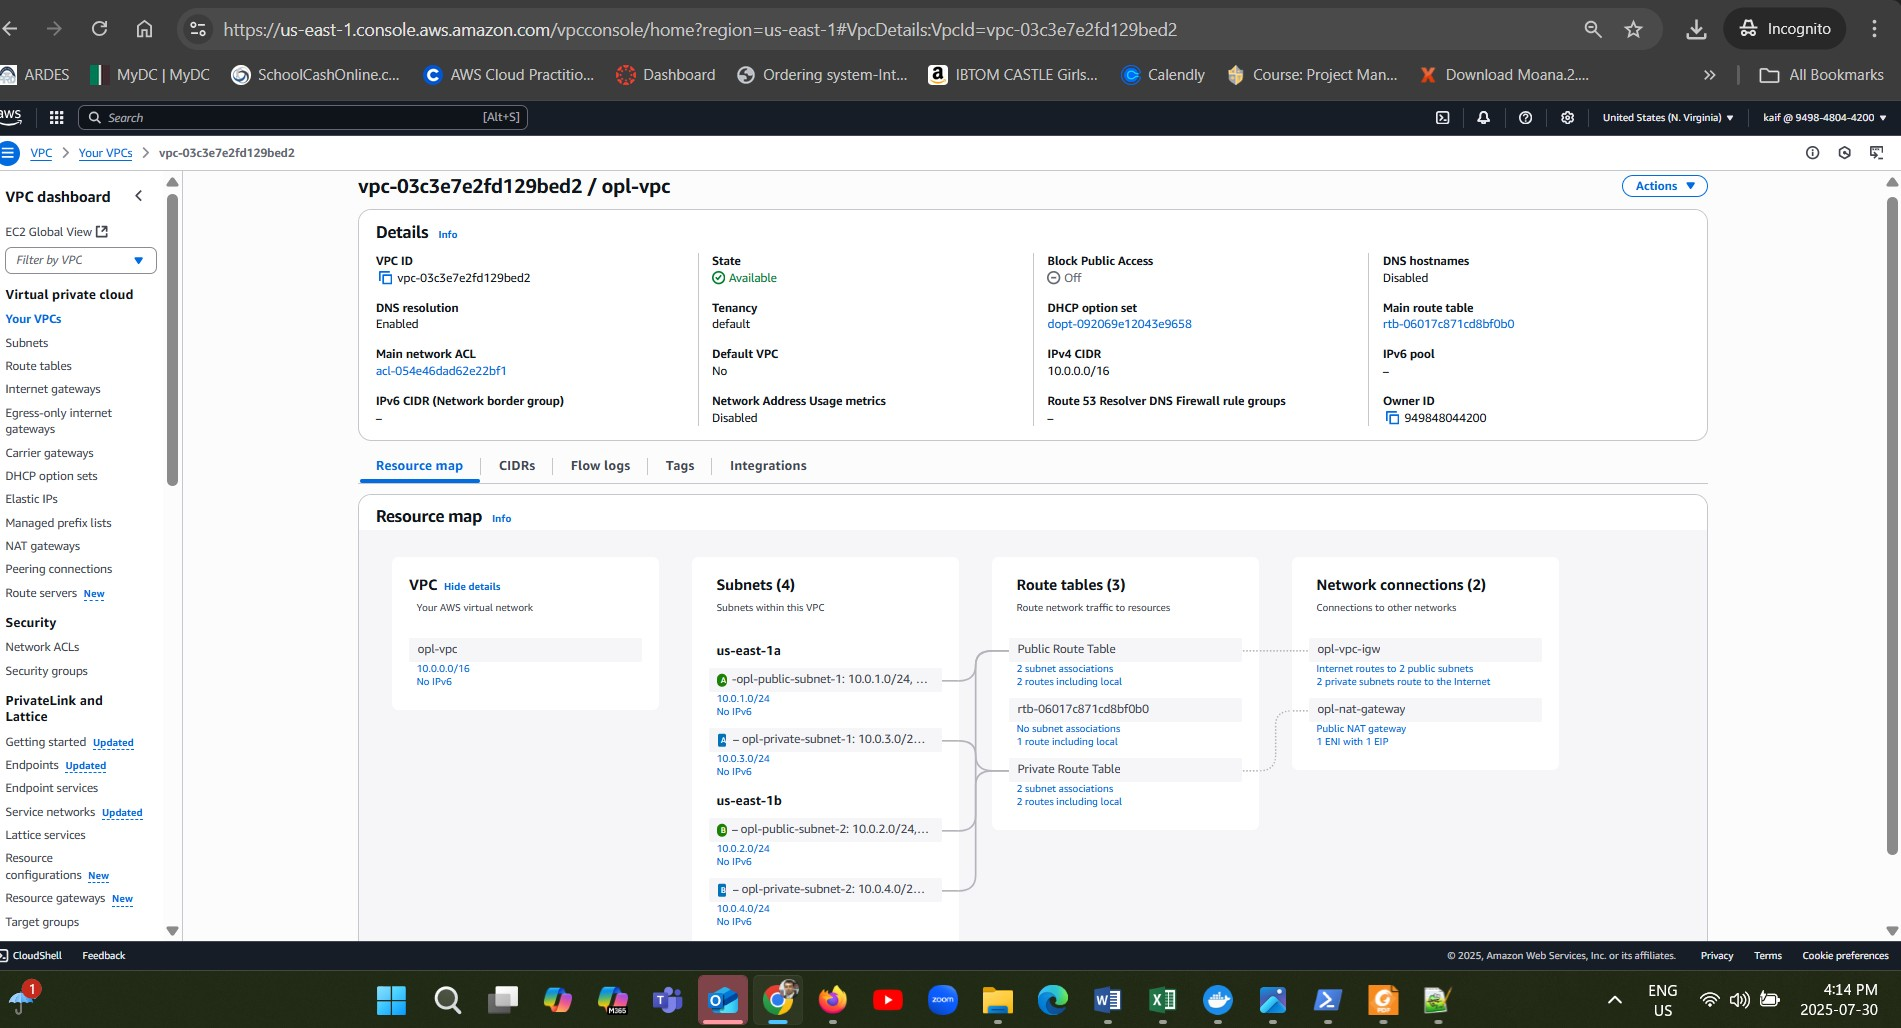
\includegraphics[width=0.8\textwidth]{vpc-subnet.jpg}
    \caption{VPC and subnet creation with CIDR blocks.}
\end{figure}
\begin{figure}[h]
    \centering
    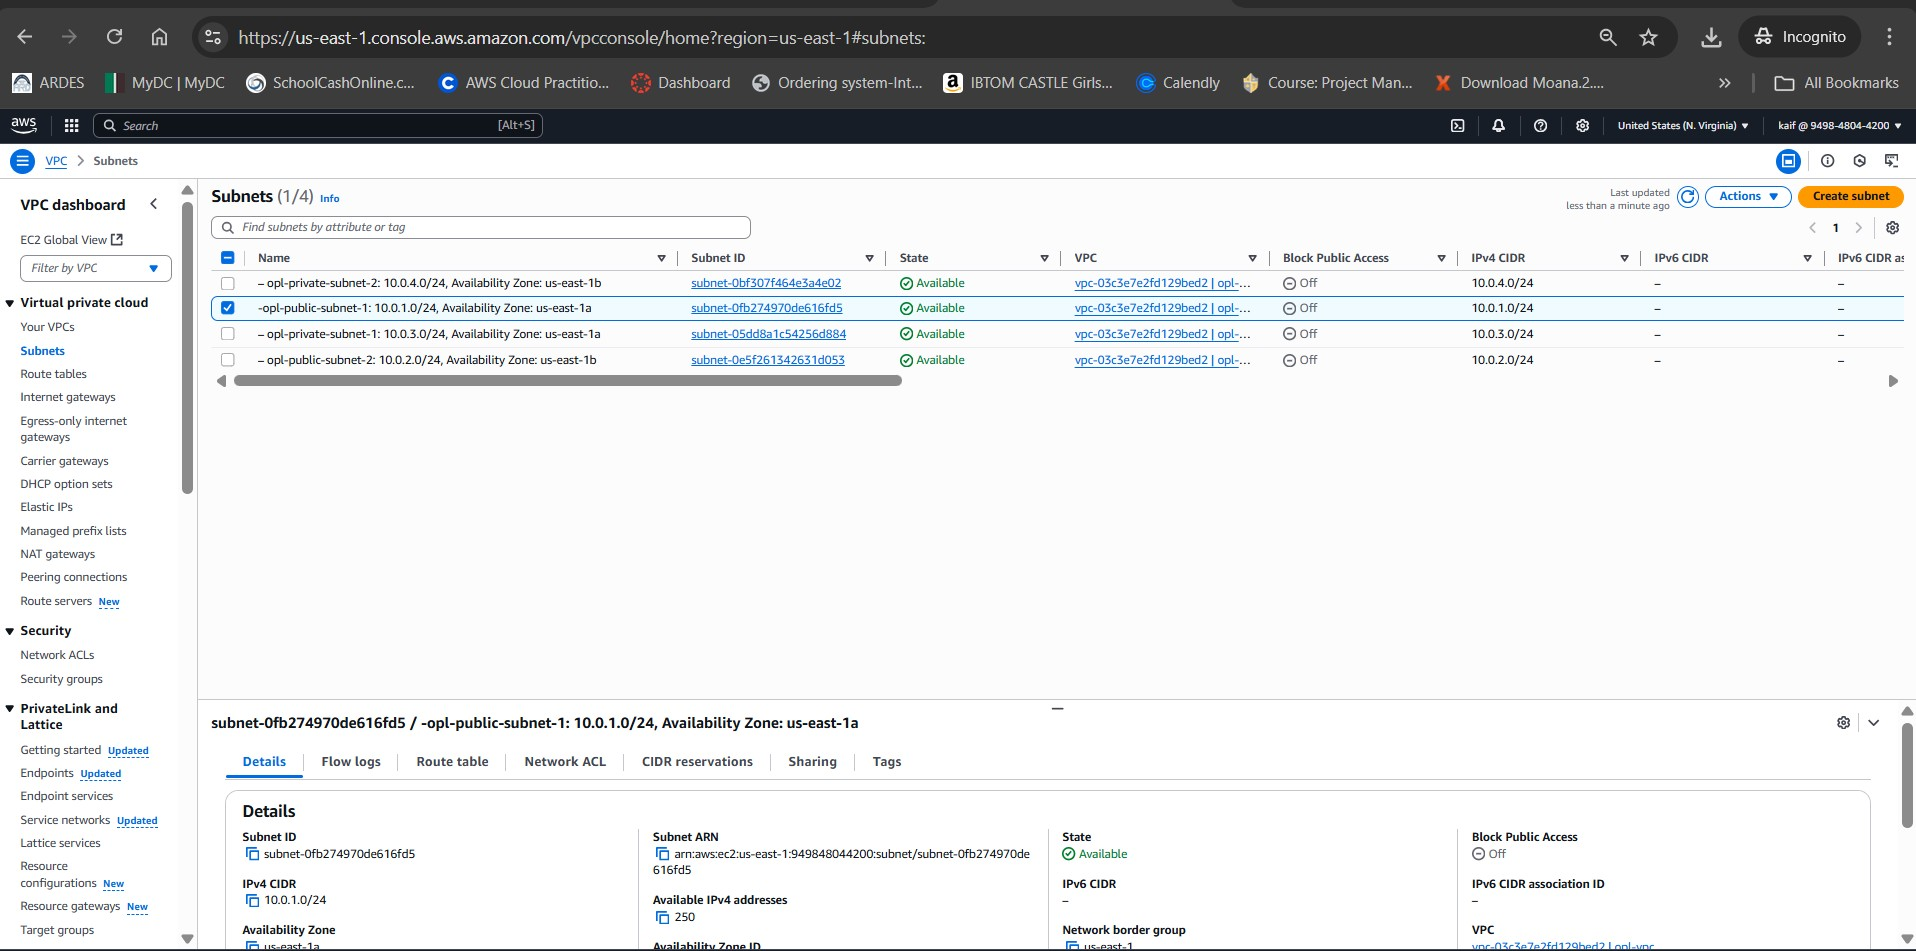
\includegraphics[width=0.8\textwidth]{subnet-config.jpg}
    \caption{Subnet configuration showing public and private subnets.}
\end{figure}
\begin{figure}[h]
    \centering
    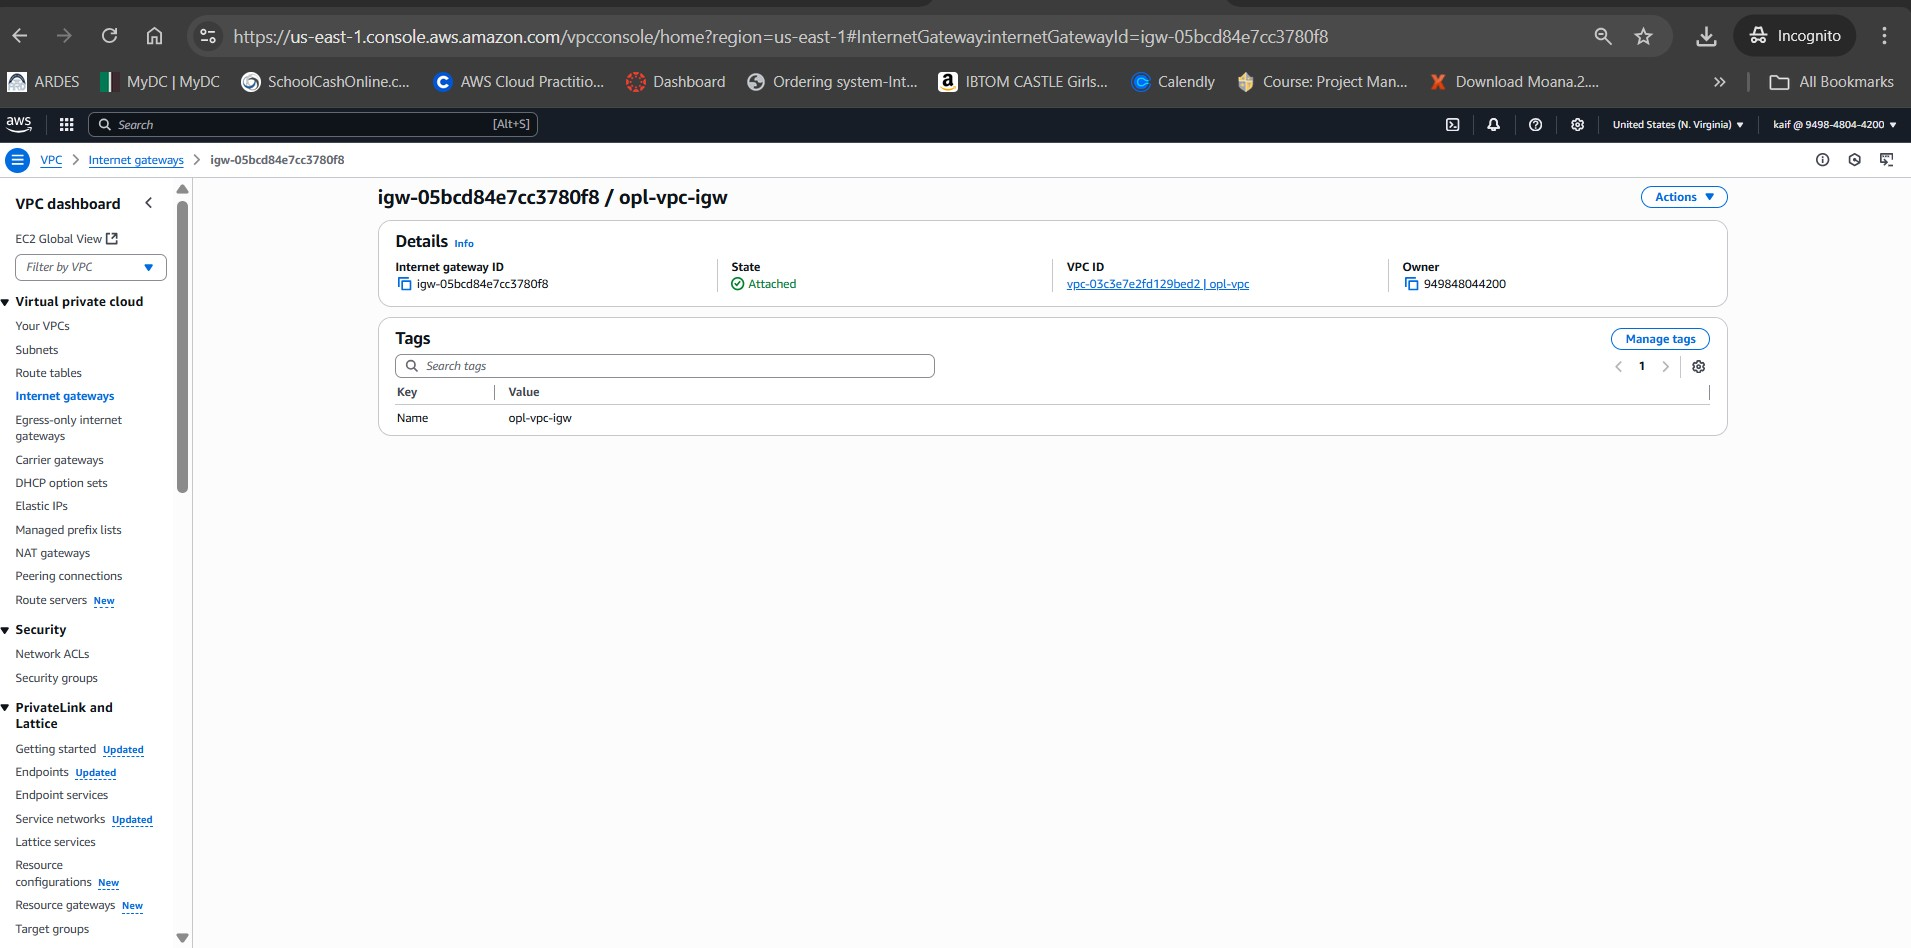
\includegraphics[width=0.8\textwidth]{internet-gateway.jpg}
    \caption{Internet Gateway attached to the VPC.}
\end{figure>
\begin{figure}[h]
    \centering
    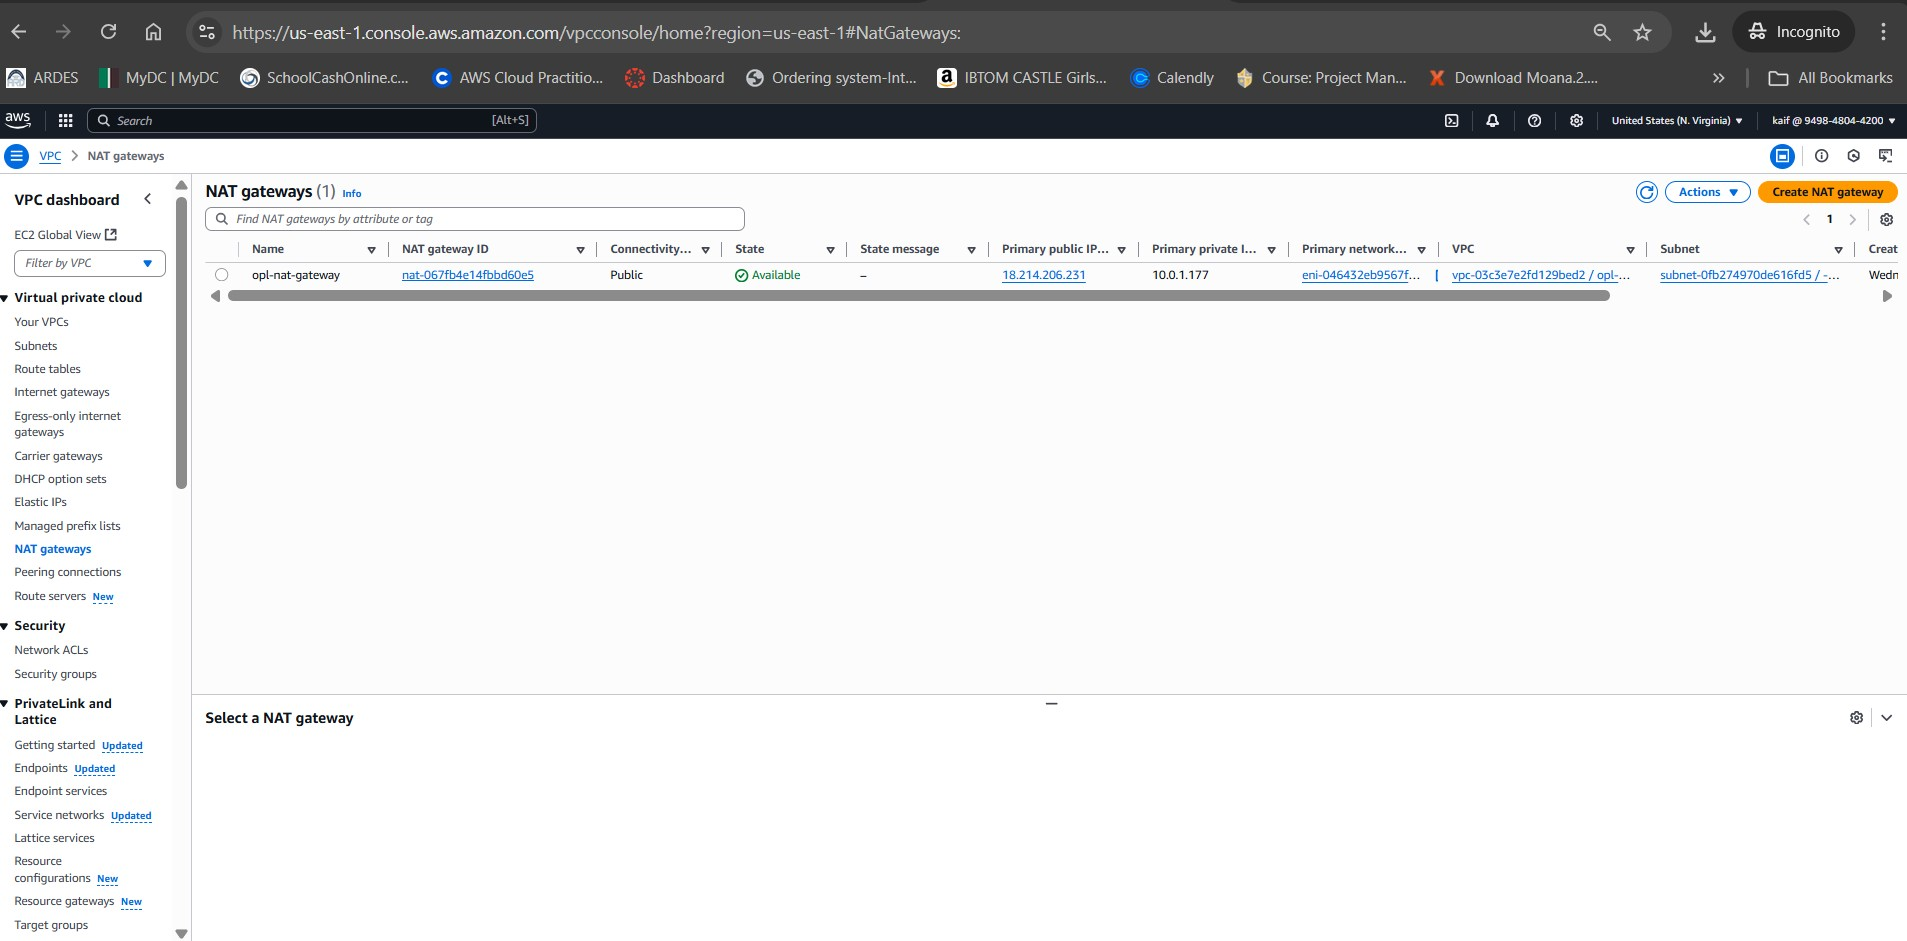
\includegraphics[width=0.8\textwidth]{Nat-gateway.jpg}
    \caption{NAT Gateway setup for private subnets.}
\end{figure>
\begin{figure}[h]
    \centering
    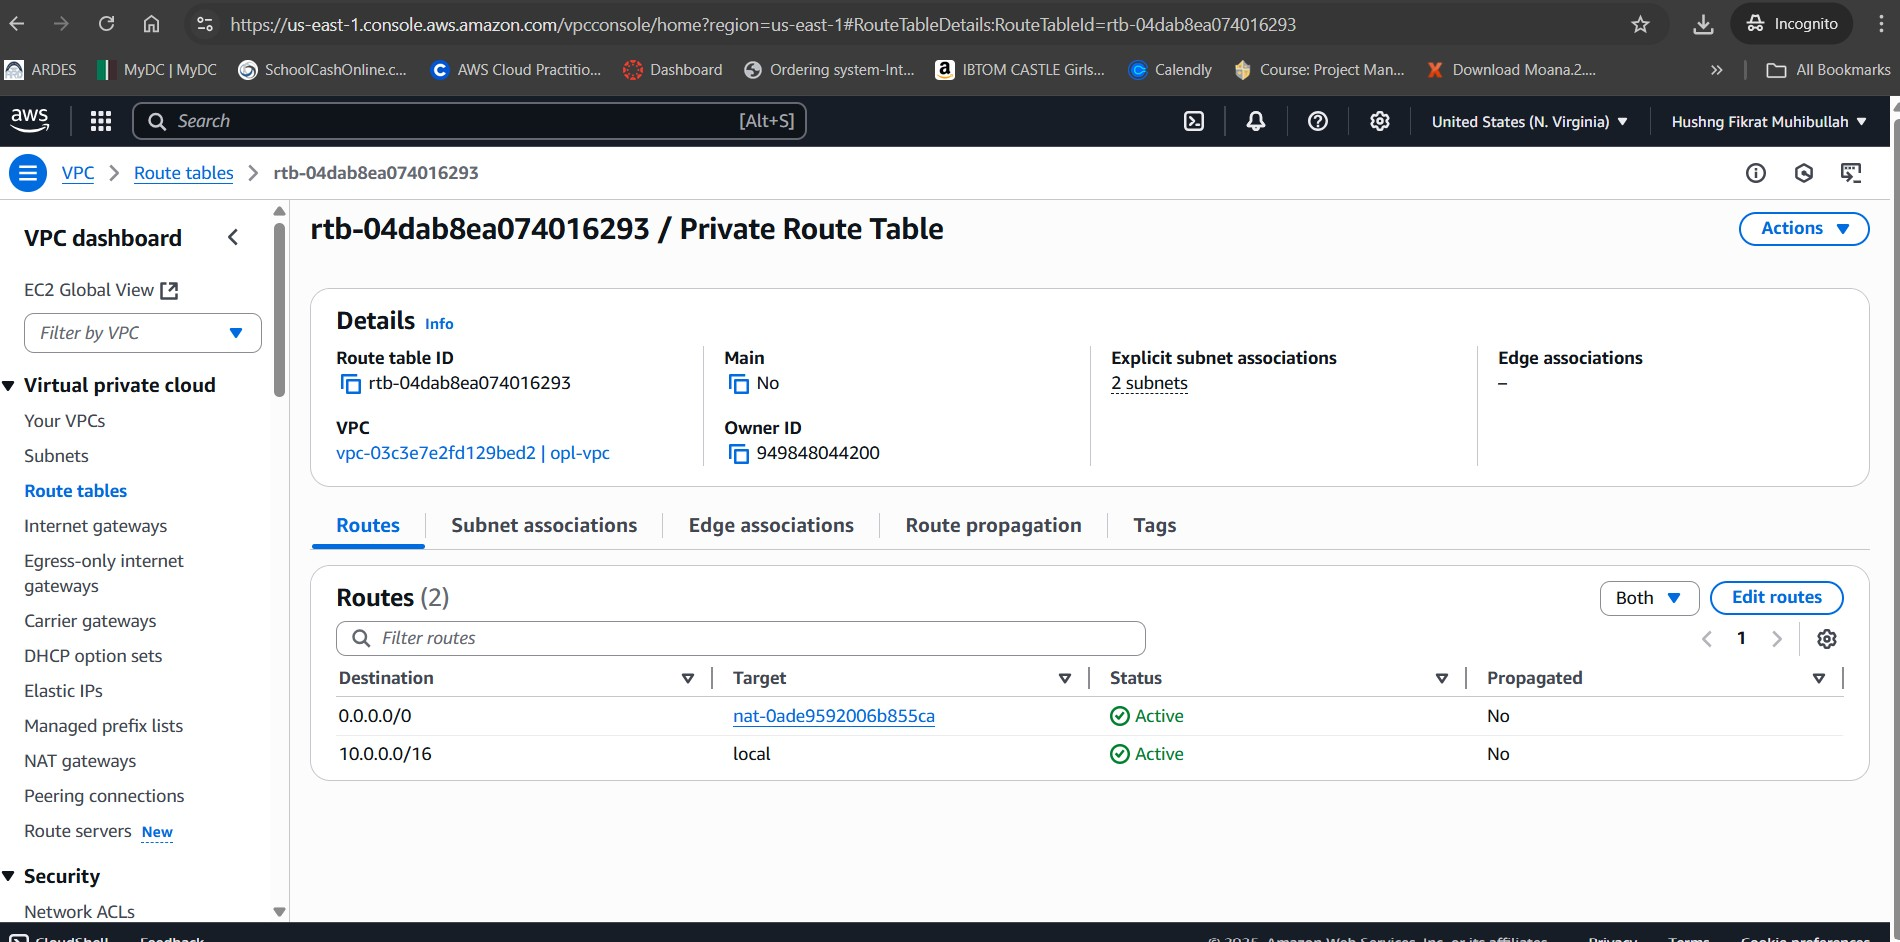
\includegraphics[width=0.8\textwidth]{routetableprivate.jpg}
    \caption{Route table for private subnets.}
\end{figure>
\begin{figure}[h]
    \centering
    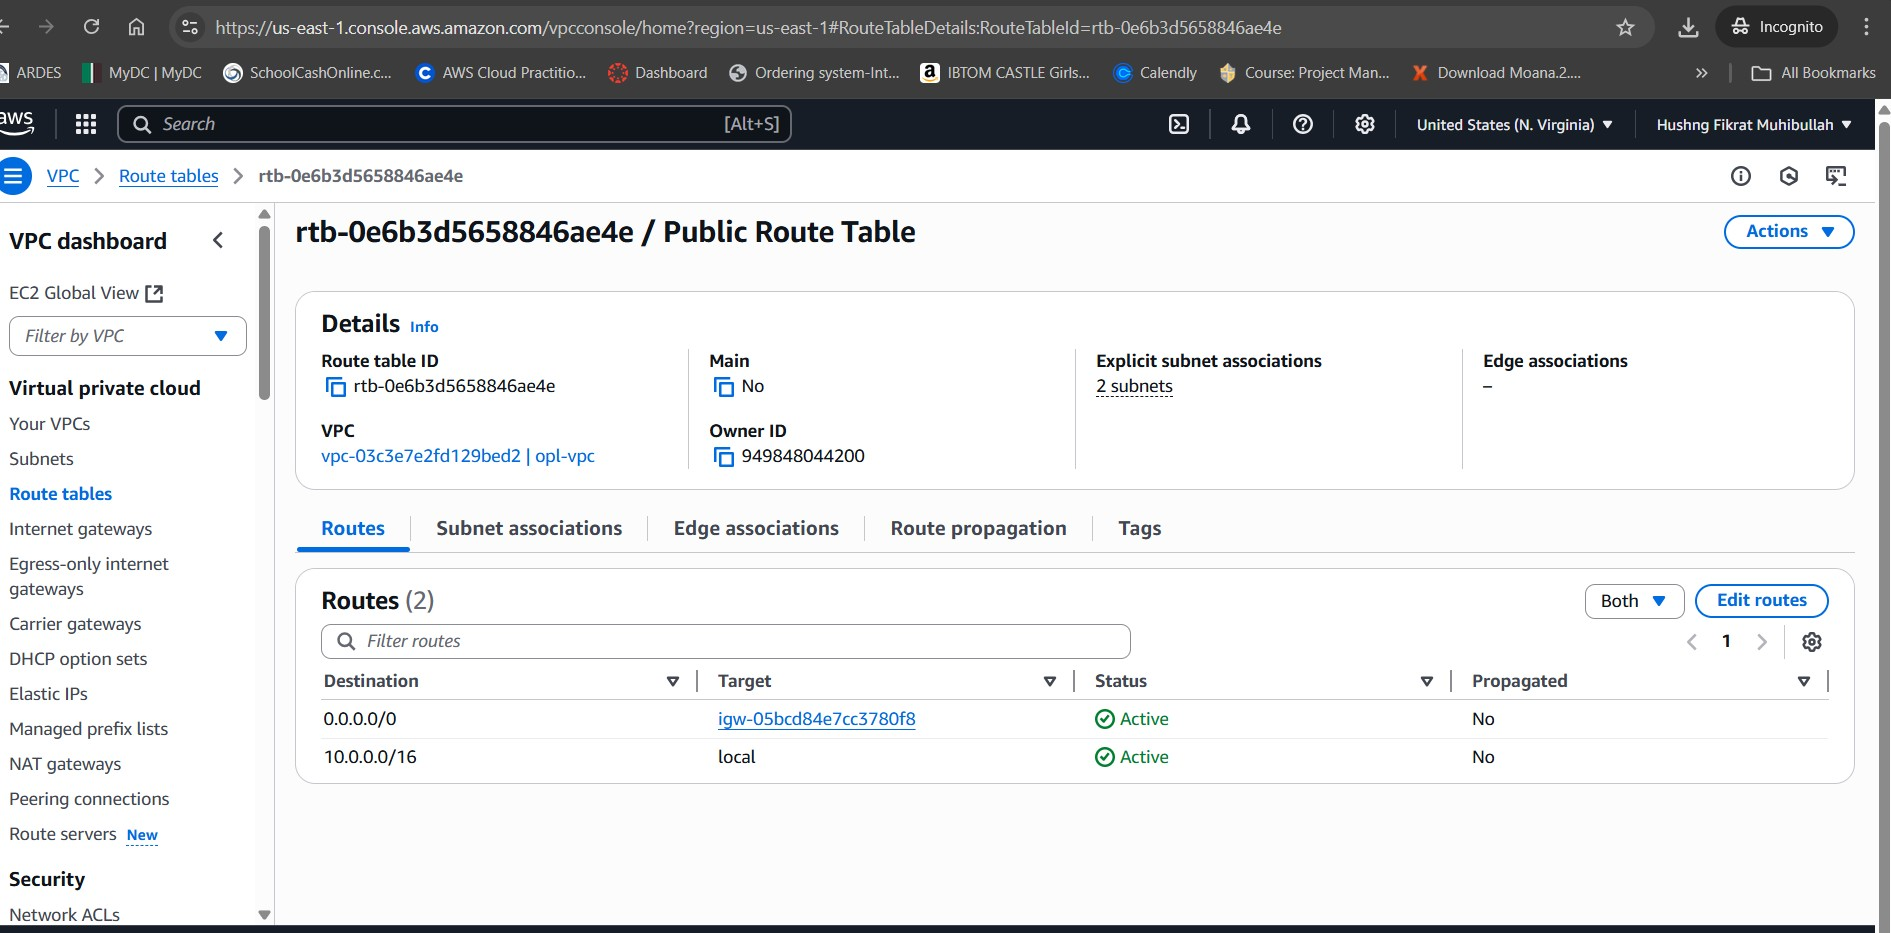
\includegraphics[width=0.8\textwidth]{routetablepublic.jpg}
    \caption{Route table for public subnets.}
\end{figure>
\begin{figure}[h]
    \centering
    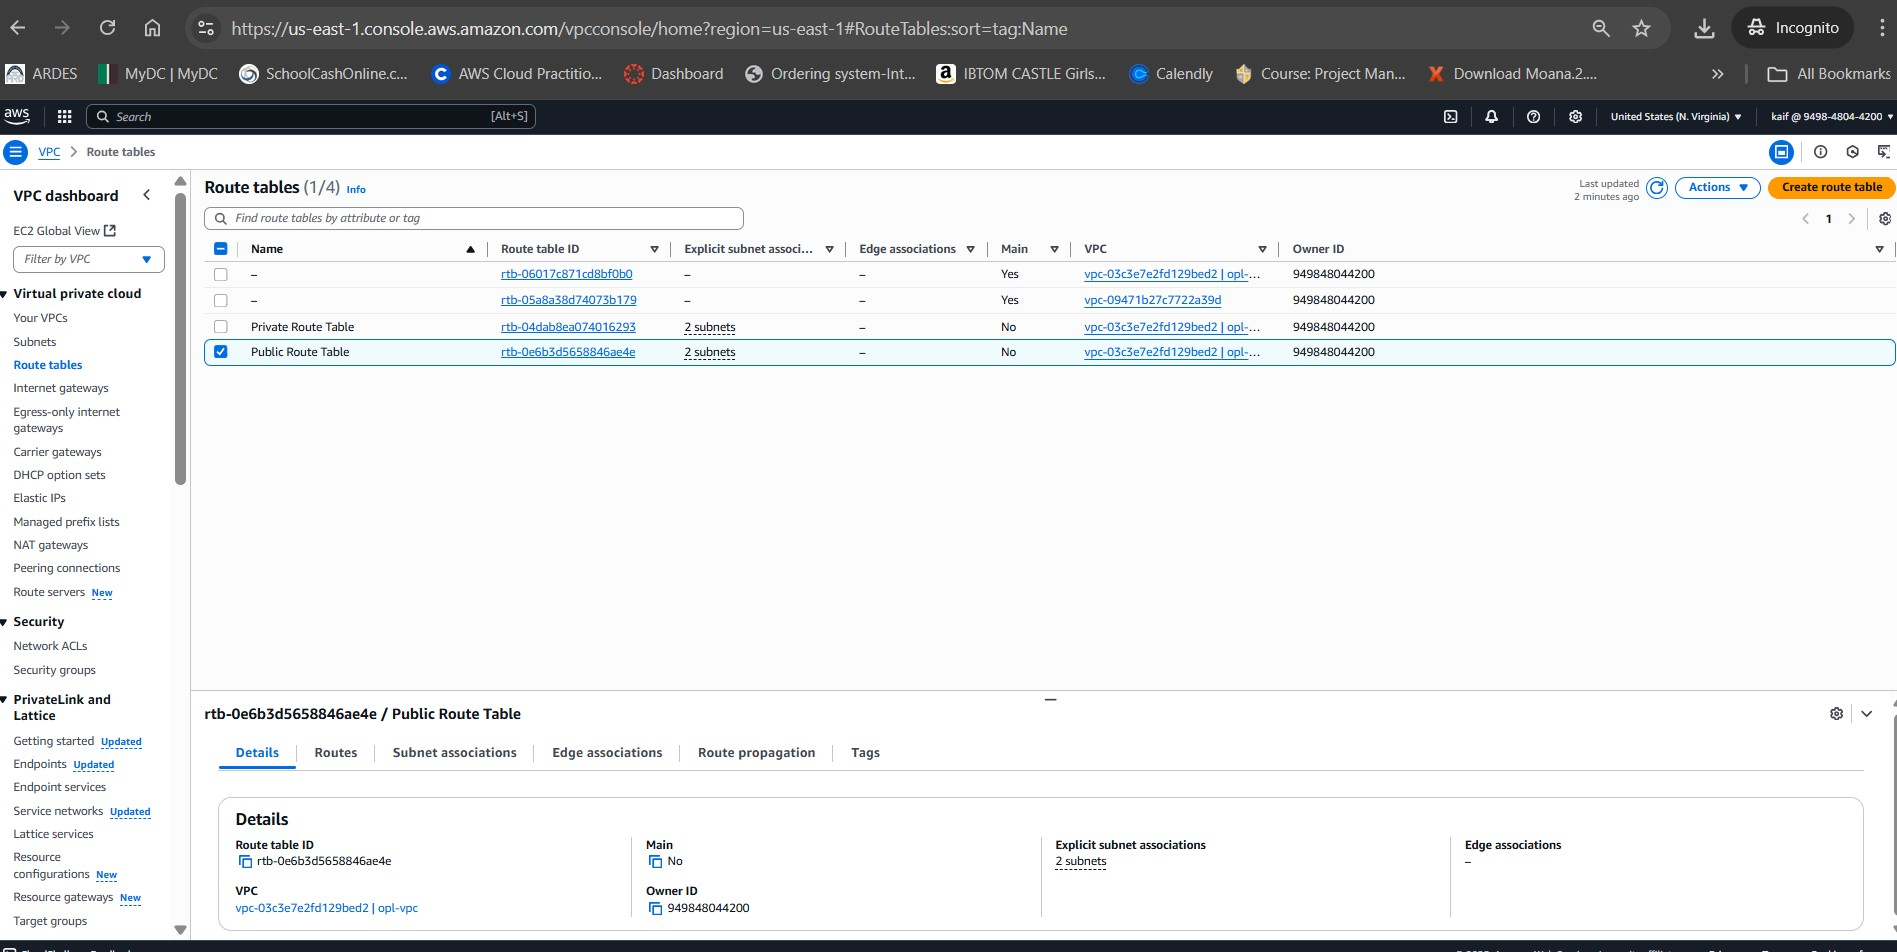
\includegraphics[width=0.8\textwidth]{route-table.jpg}
    \caption{Route table associations.}
\end{figure}
\begin{figure}[h]
    \centering
    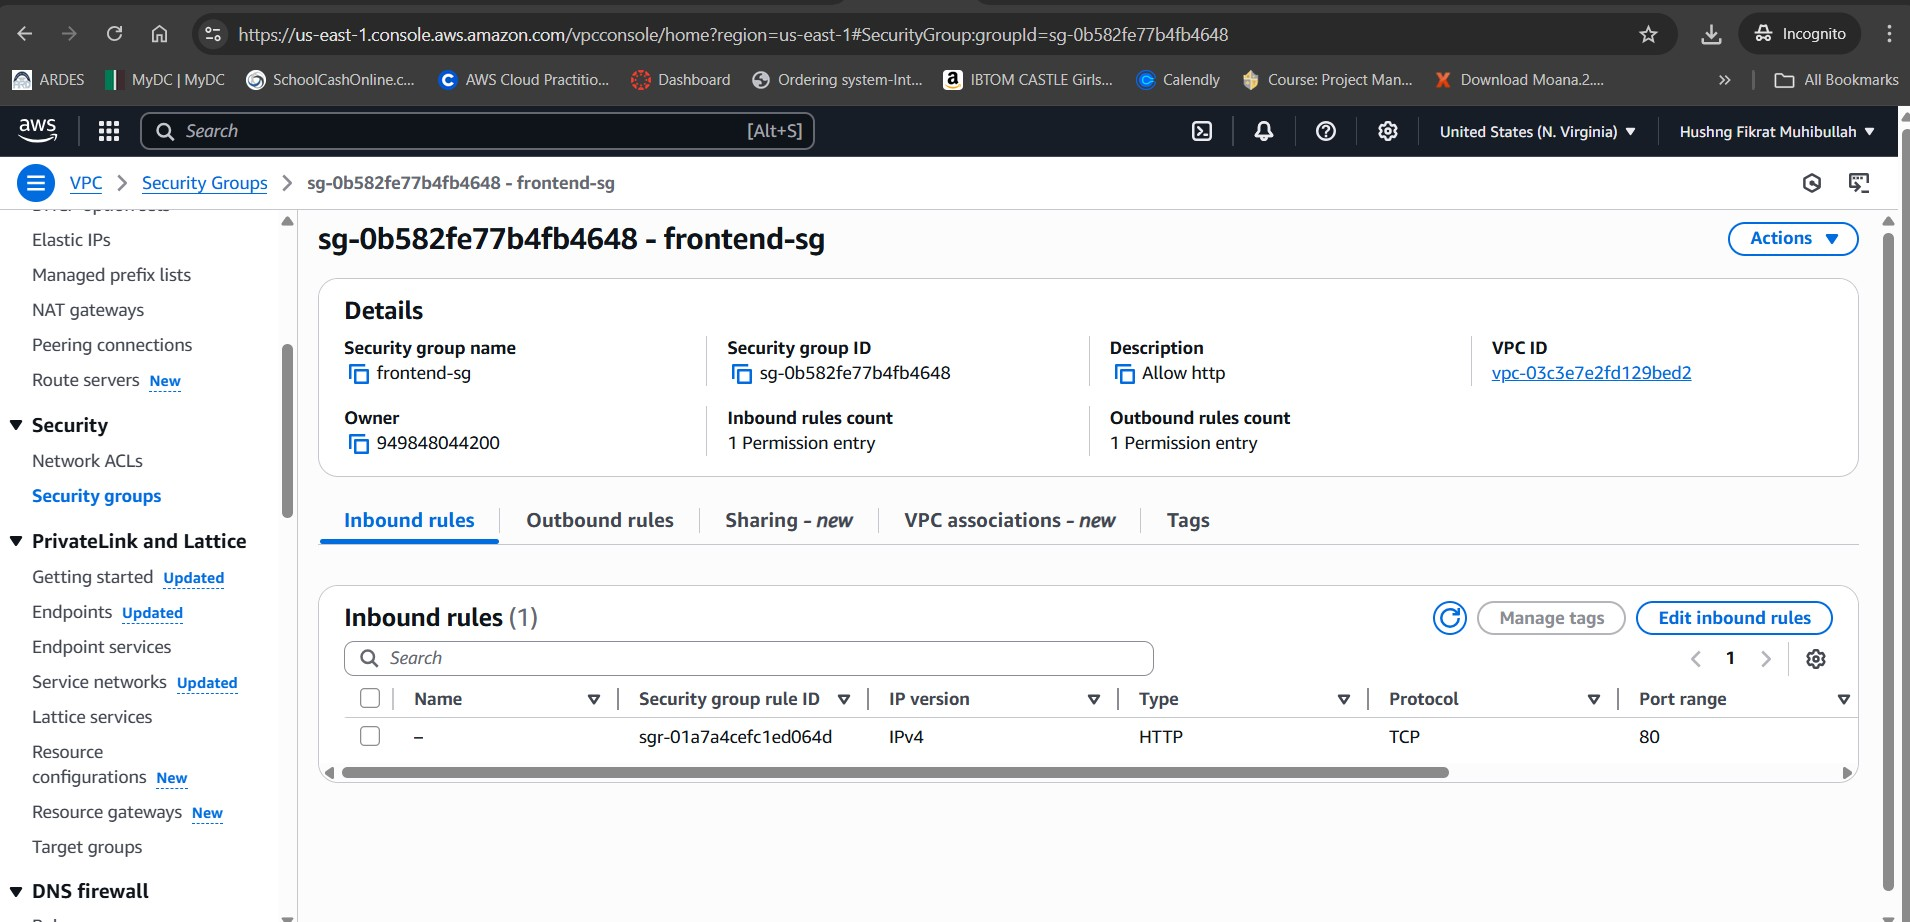
\includegraphics[width=0.8\textwidth]{sg-inbound-rule.jpg}
    \caption{Security Group inbound rule for HTTP traffic on port 80.}
\end{figure>
\begin{figure}[h]
    \centering
    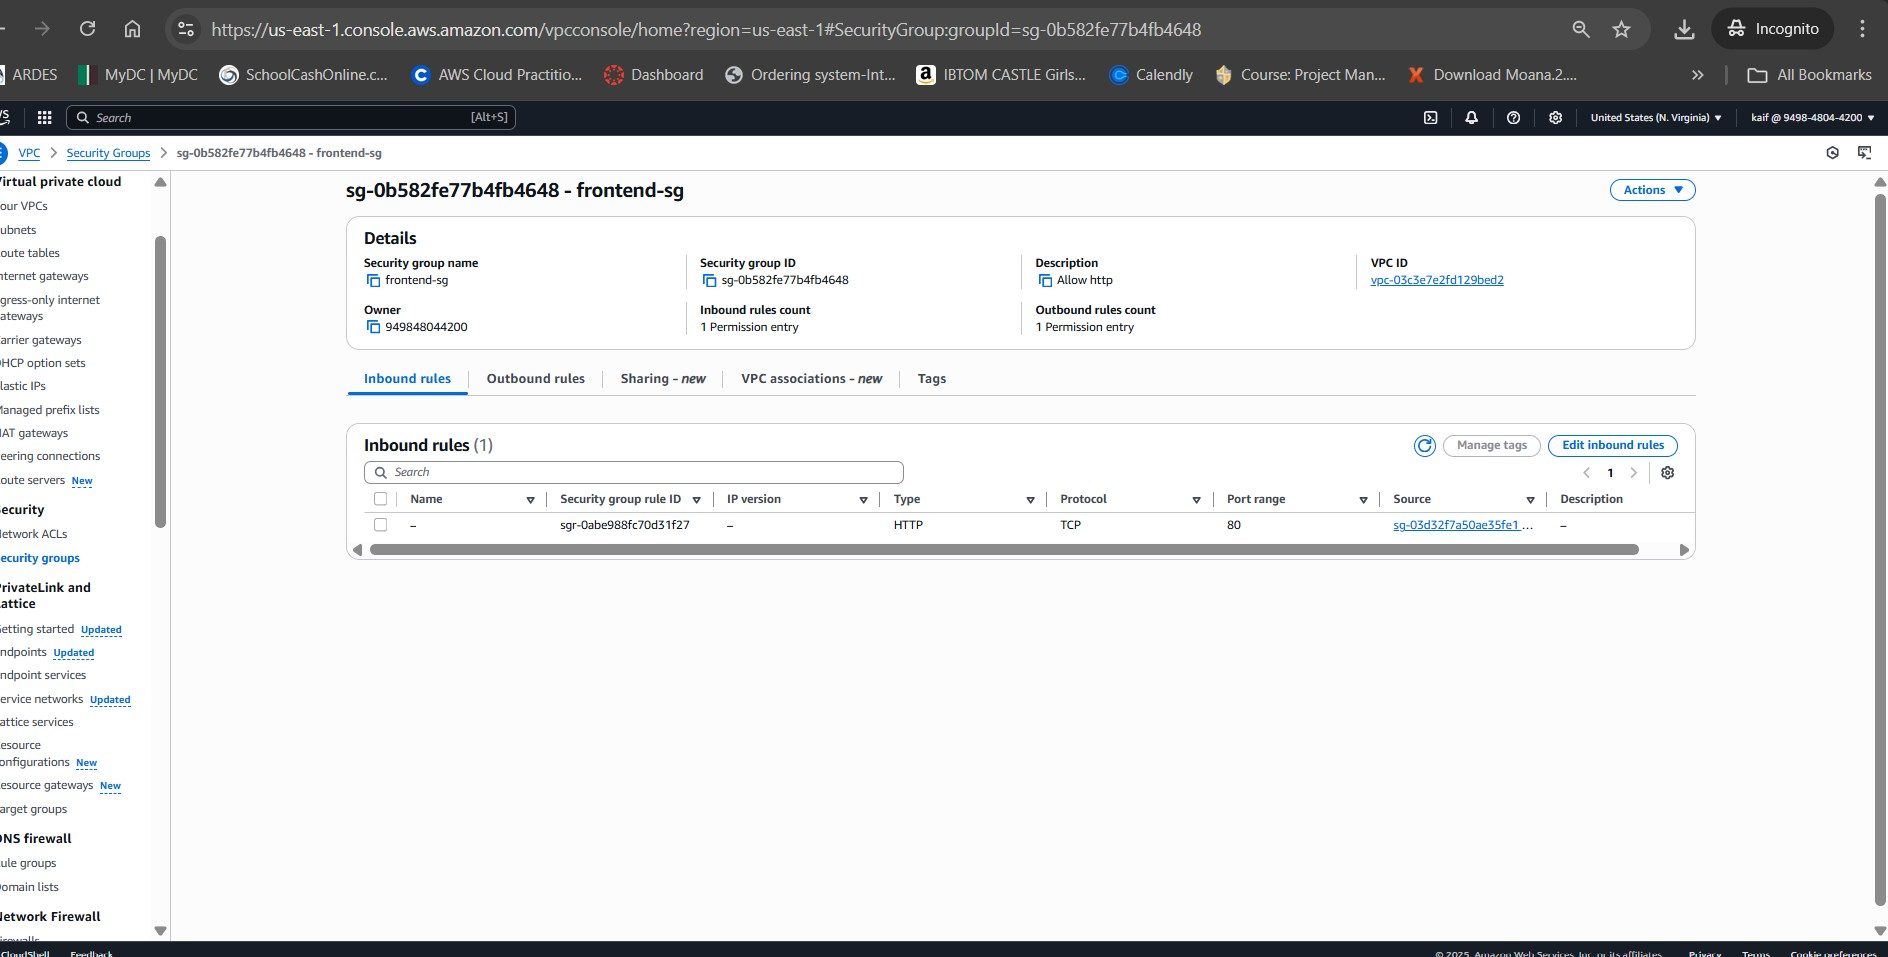
\includegraphics[width=0.8\textwidth]{frontend-sg.jpg}
    \caption{The `frontend-sg` security group for the web application.}
\end{figure>

\subsection{ECS Cluster and Service Deployment}
\begin{figure}[h]
    \centering
    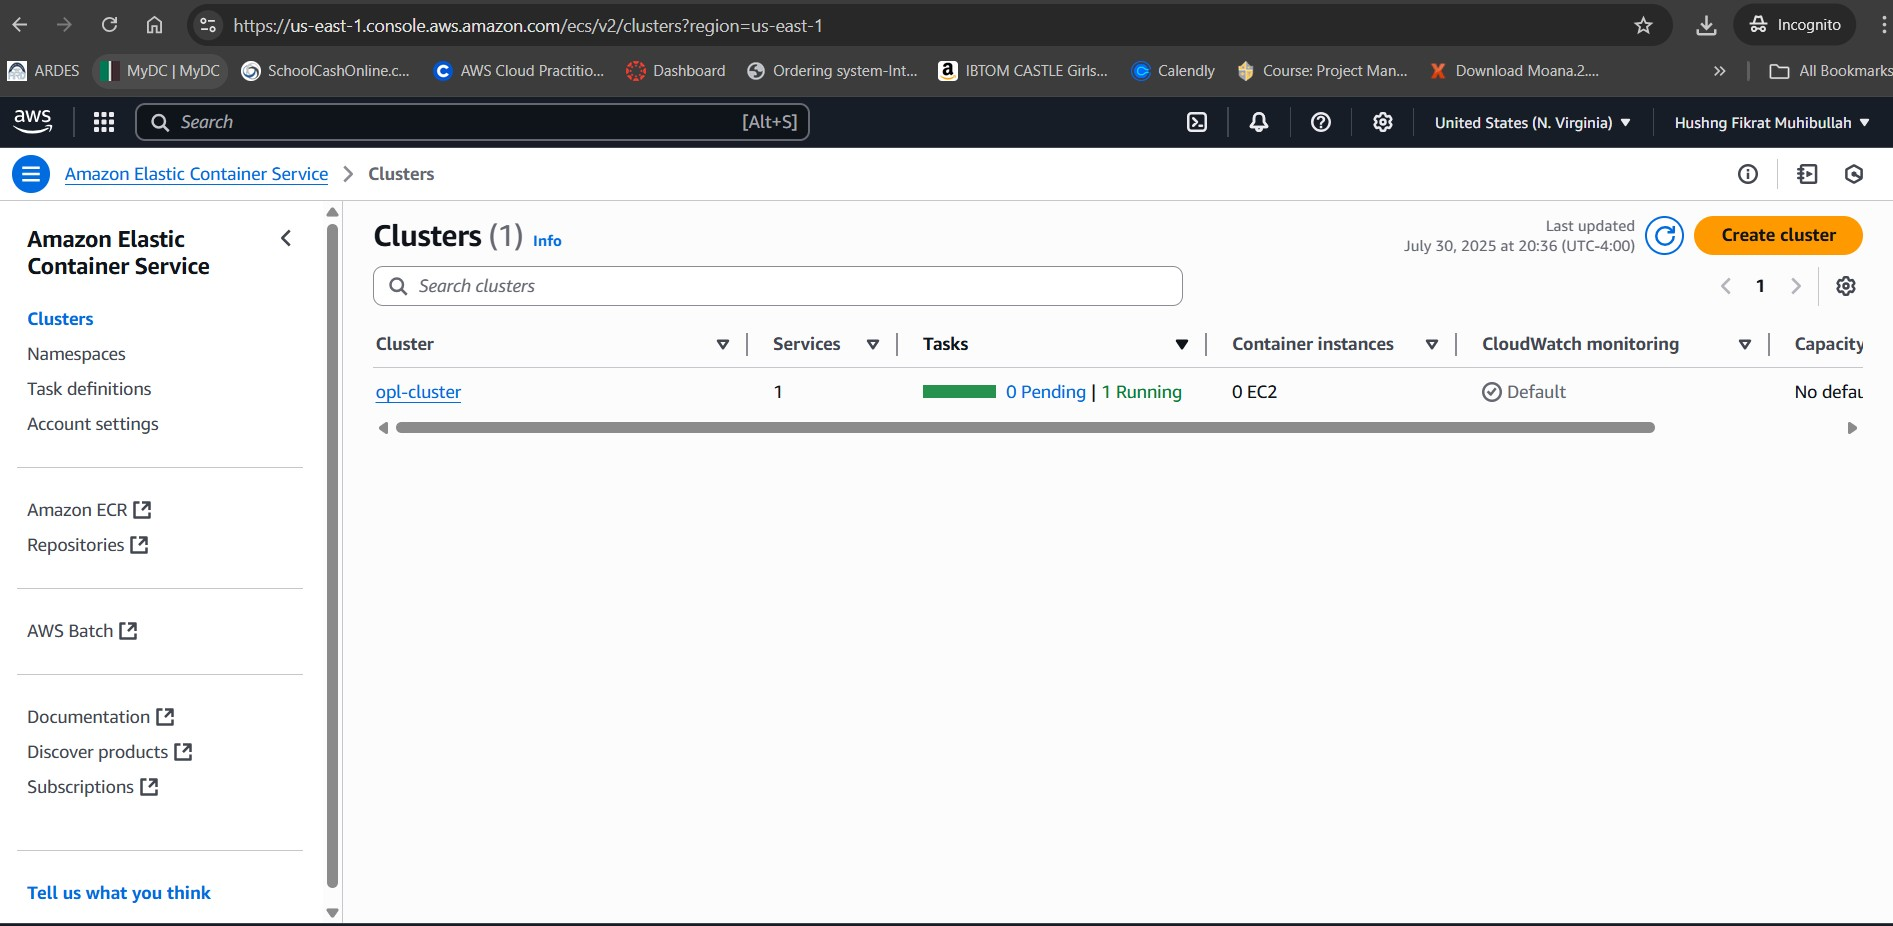
\includegraphics[width=0.8\textwidth]{cluster_1.jpg}
    \caption{The ECS cluster creation process.}
\end{figure}
\begin{figure}[h]
    \centering
    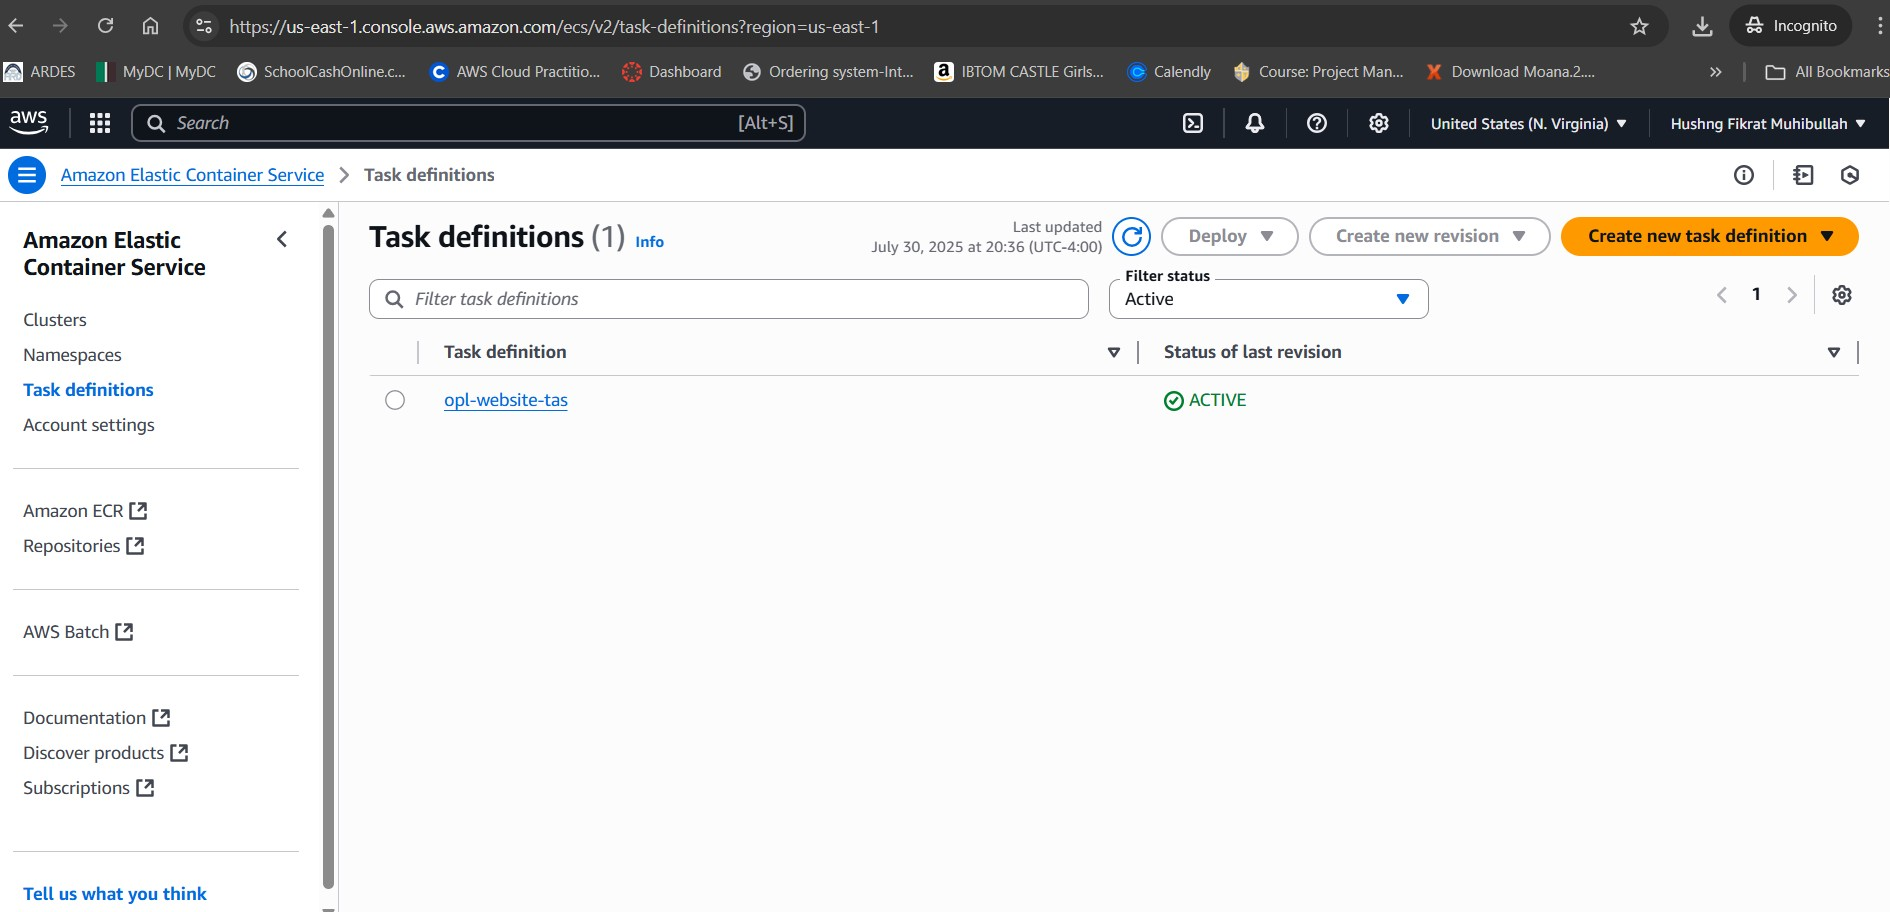
\includegraphics[width=0.8\textwidth]{cluster_2.jpg}
    \caption{ECS cluster with Fargate infrastructure.}
\end{figure>
\begin{figure}[h]
    \centering
    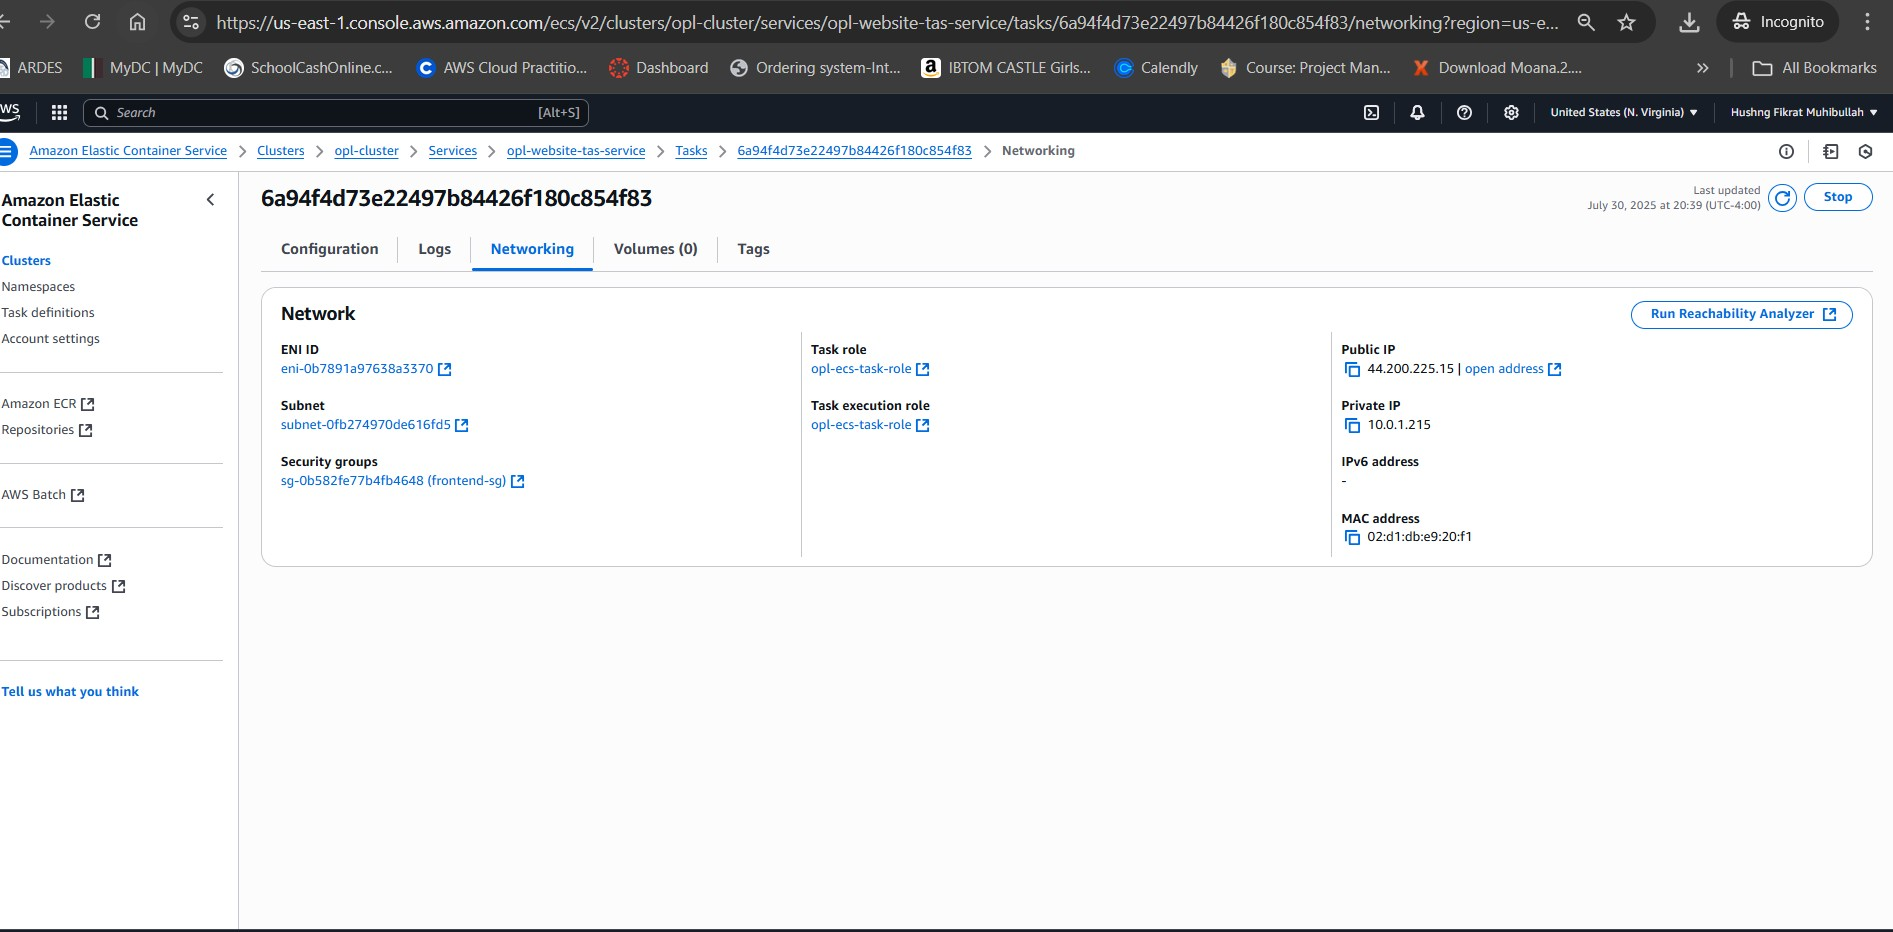
\includegraphics[width=0.8\textwidth]{Cluster_network.jpg}
    \caption{Network configuration for the ECS cluster.}
\end{figure>
\begin{figure}[h]
    \centering
    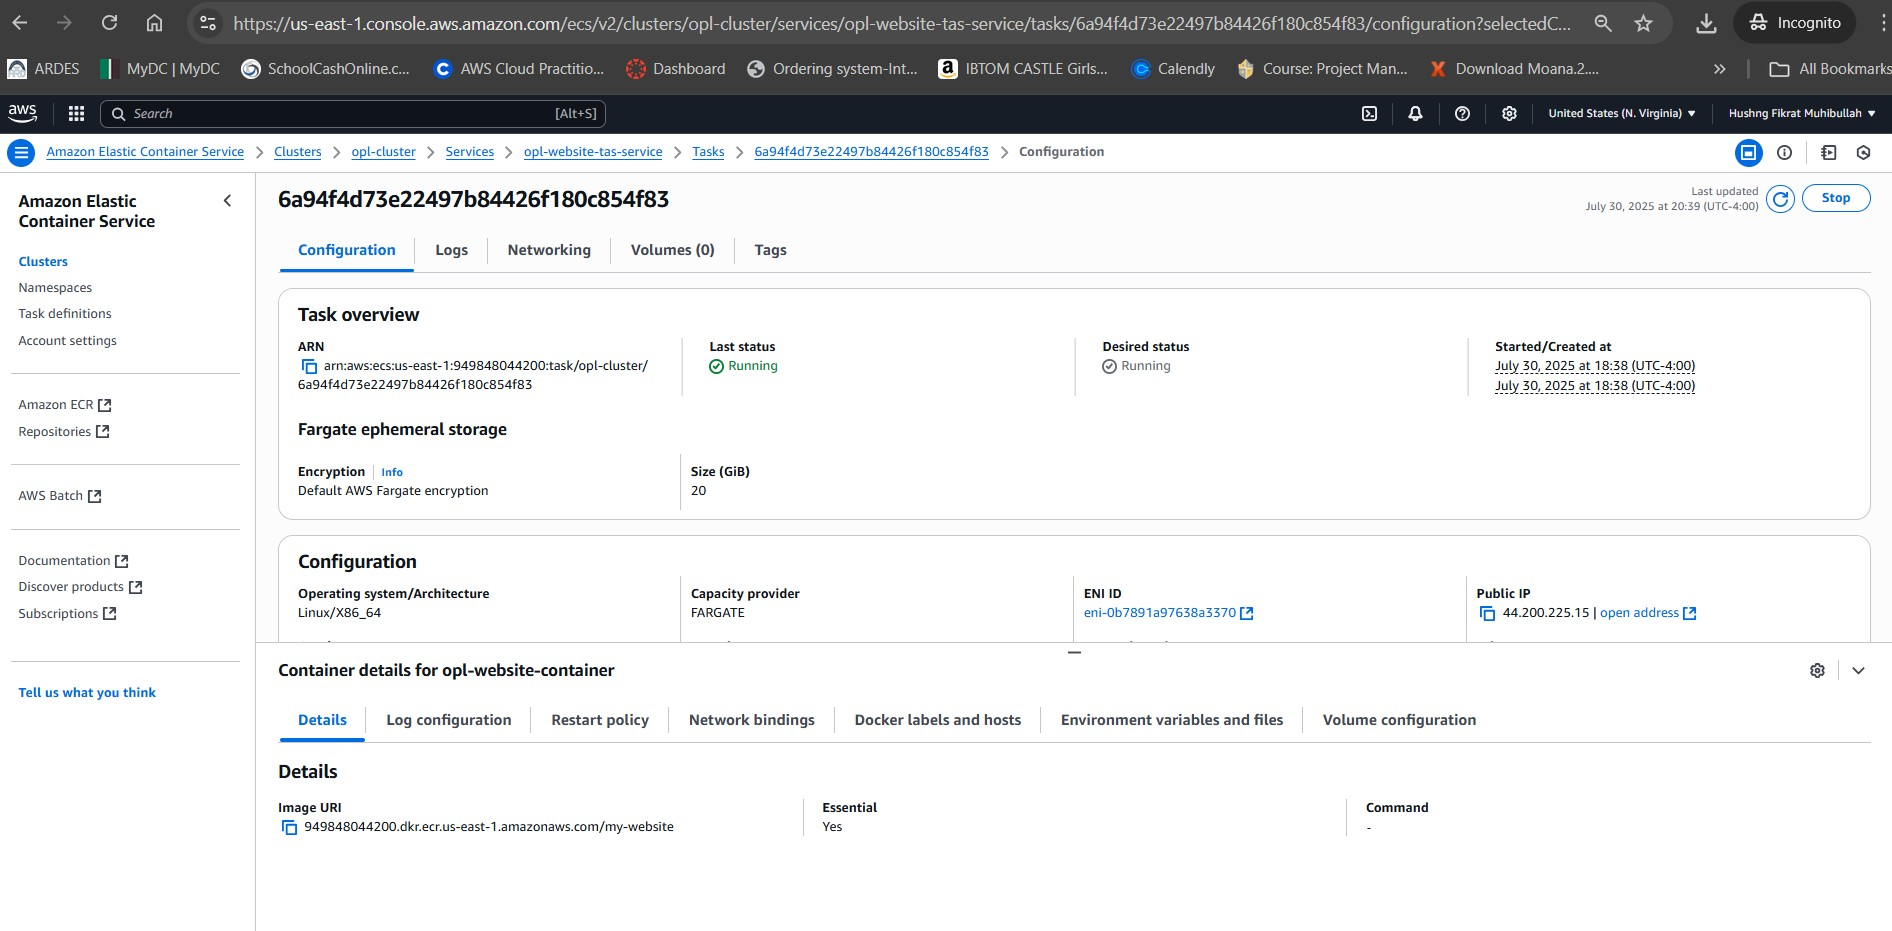
\includegraphics[width=0.8\textwidth]{inside_cluster.jpg}
    \caption{The service running inside the ECS cluster.}
\end{figure>
\begin{figure}[h]
    \centering
    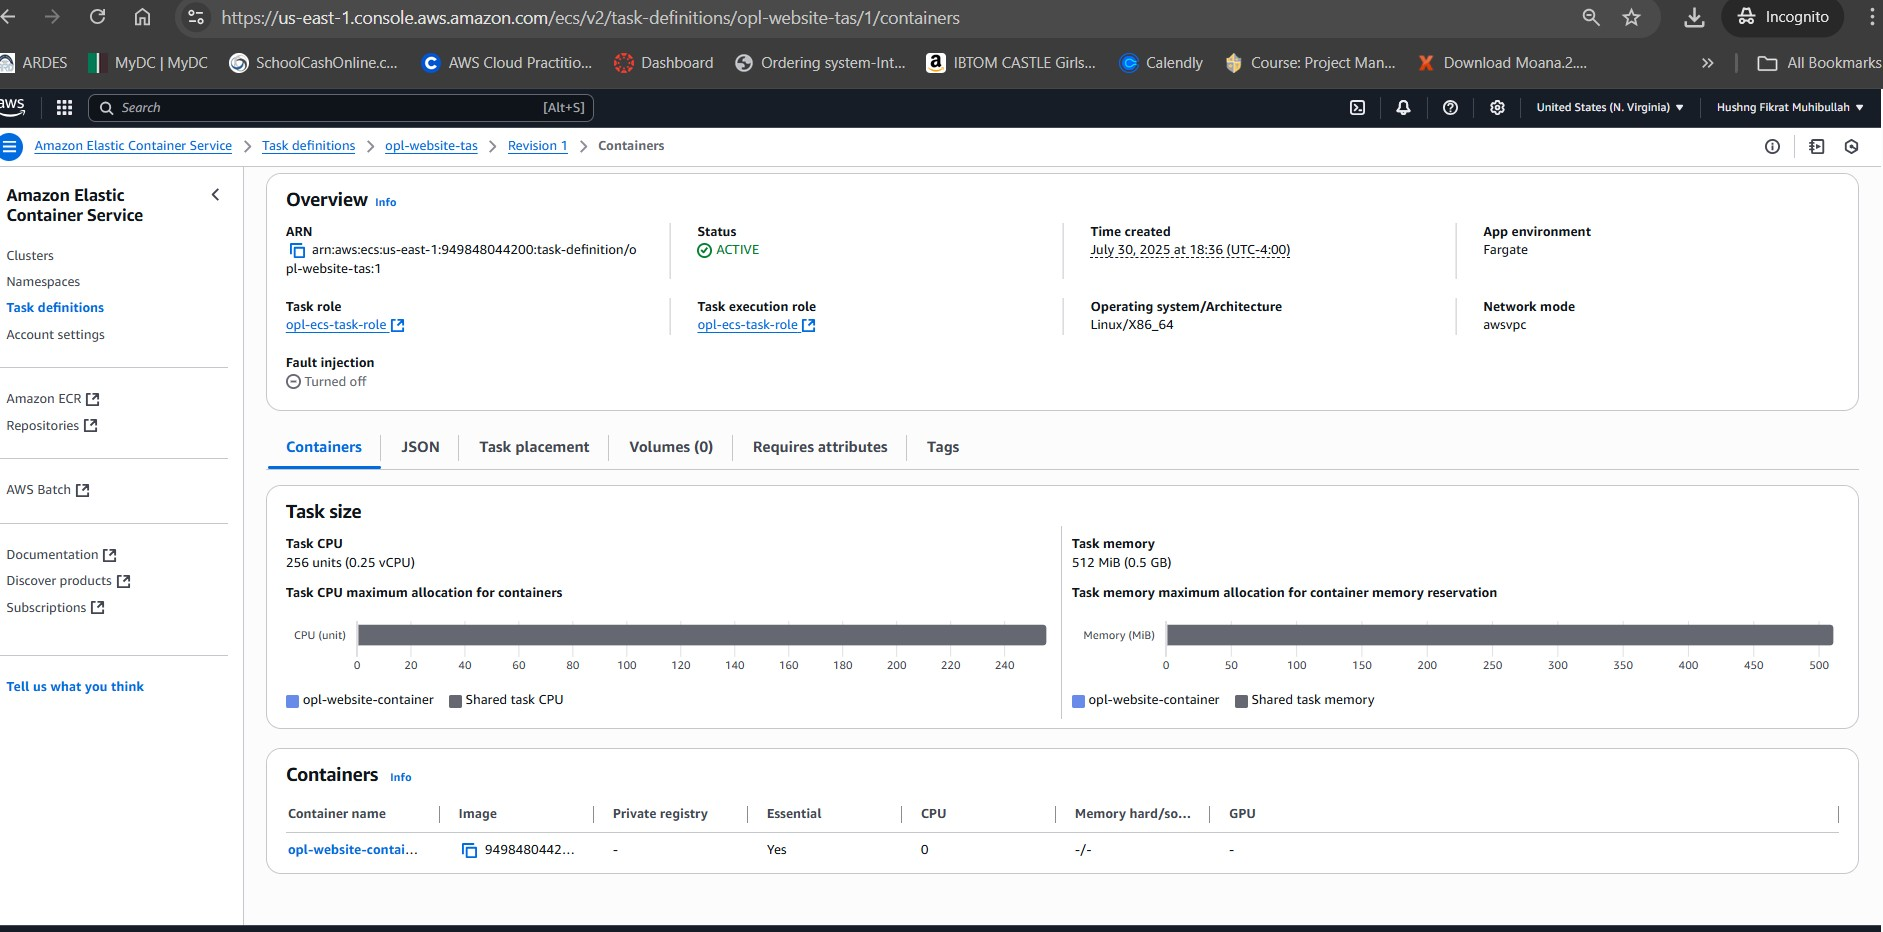
\includegraphics[width=0.8\textwidth]{task-definition.jpg}
    \caption{Creation of the task definition.}
\end{figure>
\begin{figure}[h]
    \centering
    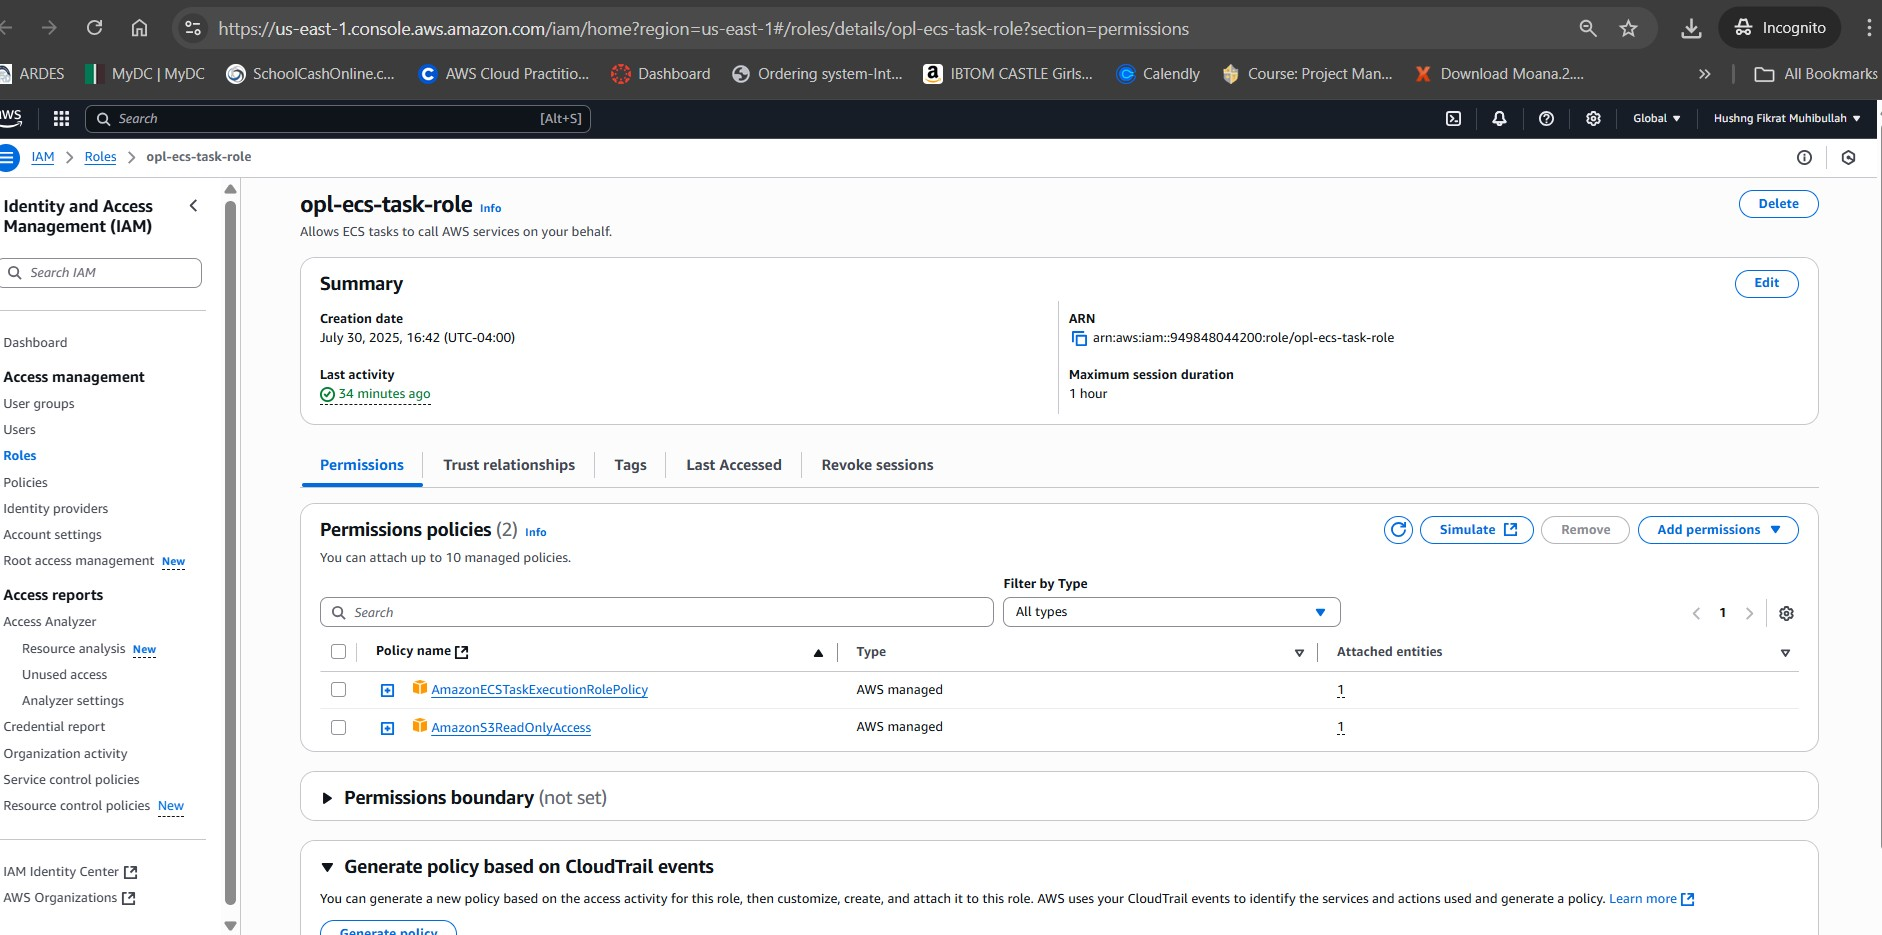
\includegraphics[width=0.8\textwidth]{task-roles.jpg}
    \caption{IAM task role assignment for the task definition.}
\end{figure}
\begin{figure}[h]
    \centering
    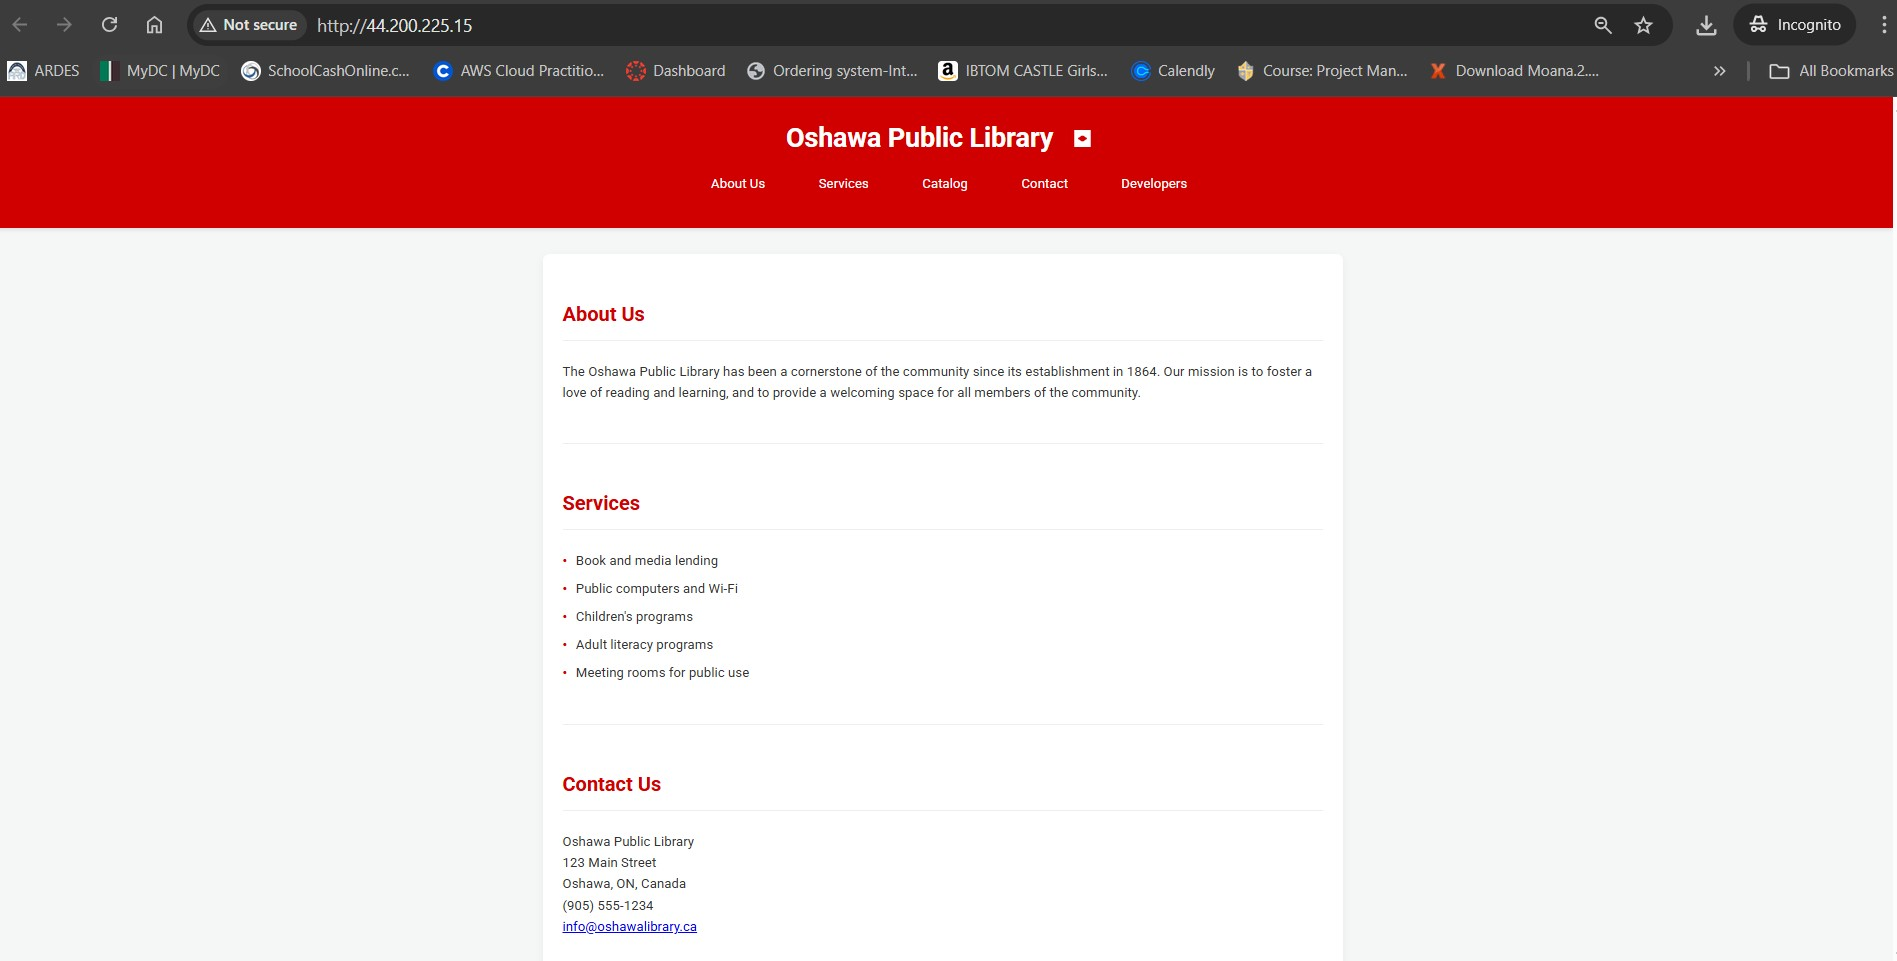
\includegraphics[width=0.8\textwidth]{runningwebsitefrompiblicip.jpg}
    \caption{The website successfully running from the public IP of the ECS task.}
\end{figure}
\begin{figure}[h]
    \centering
    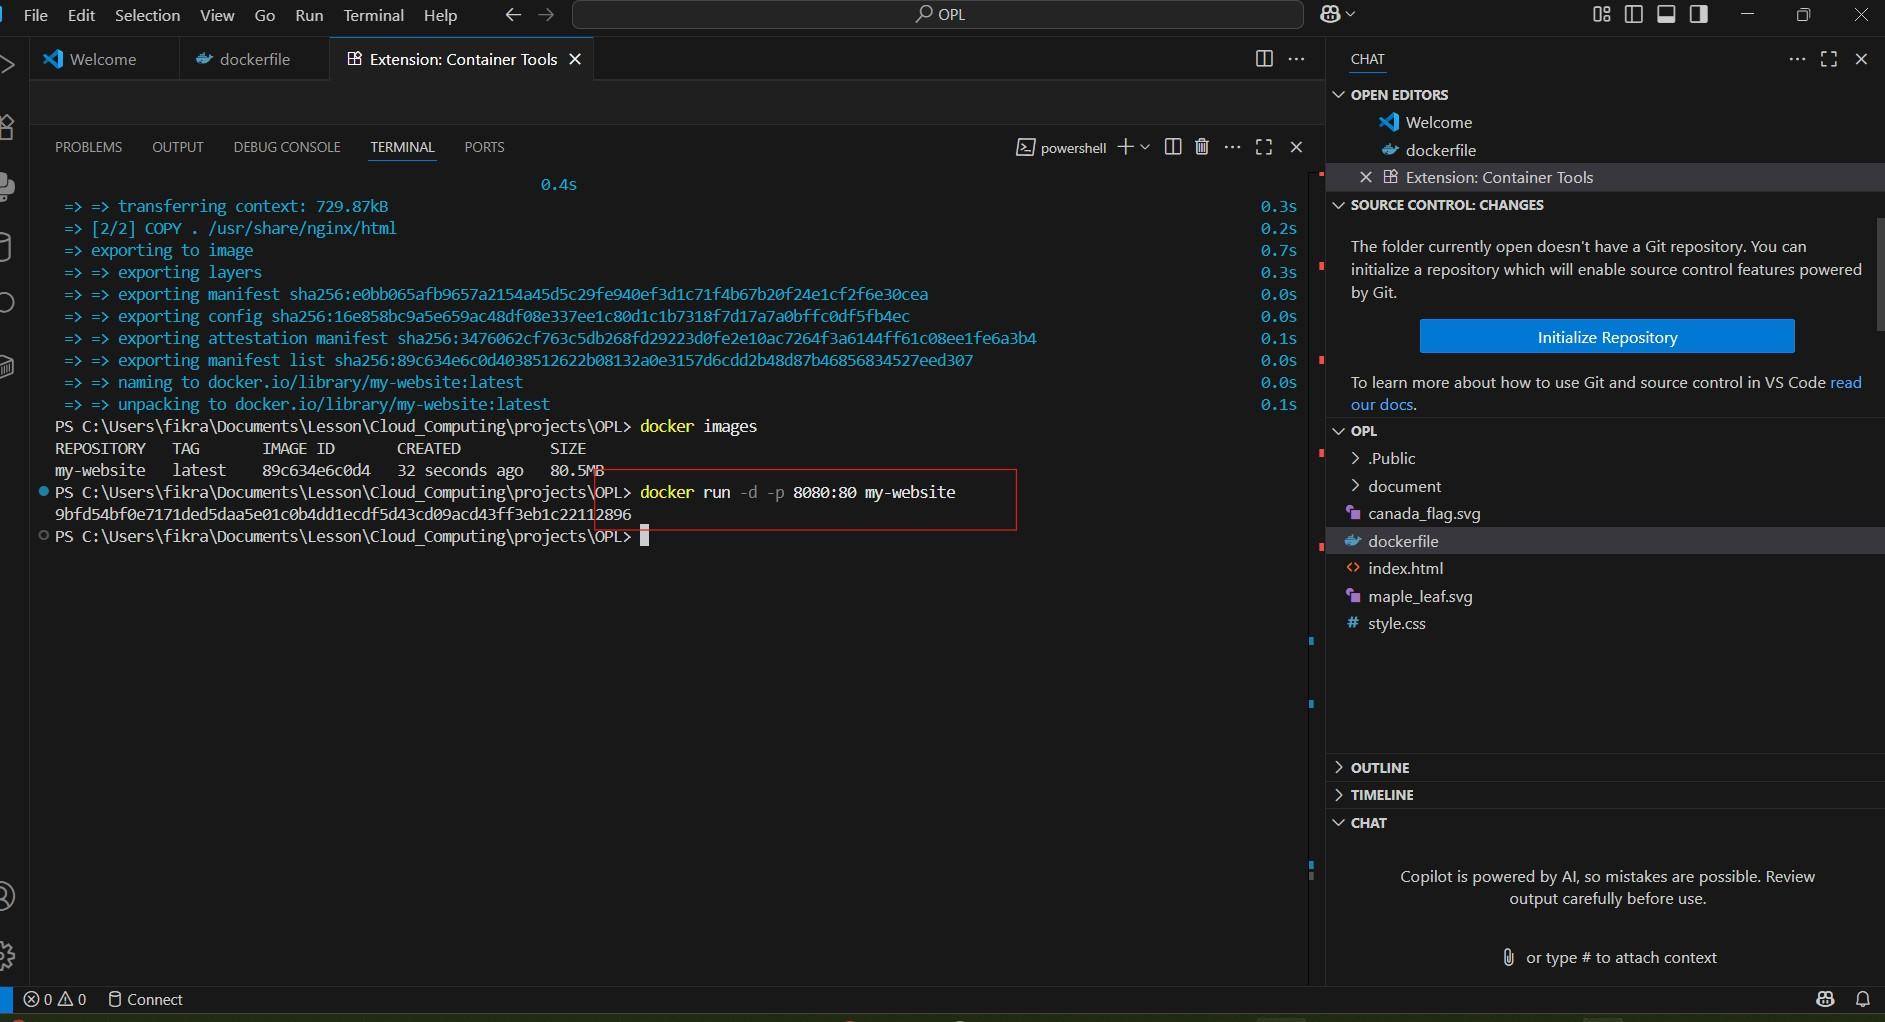
\includegraphics[width=0.8\textwidth]{app_deployed_8080.jpg}
    \caption{The deployed application is accessible.}
\end{figure>
\begin{figure}[h]
    \centering
    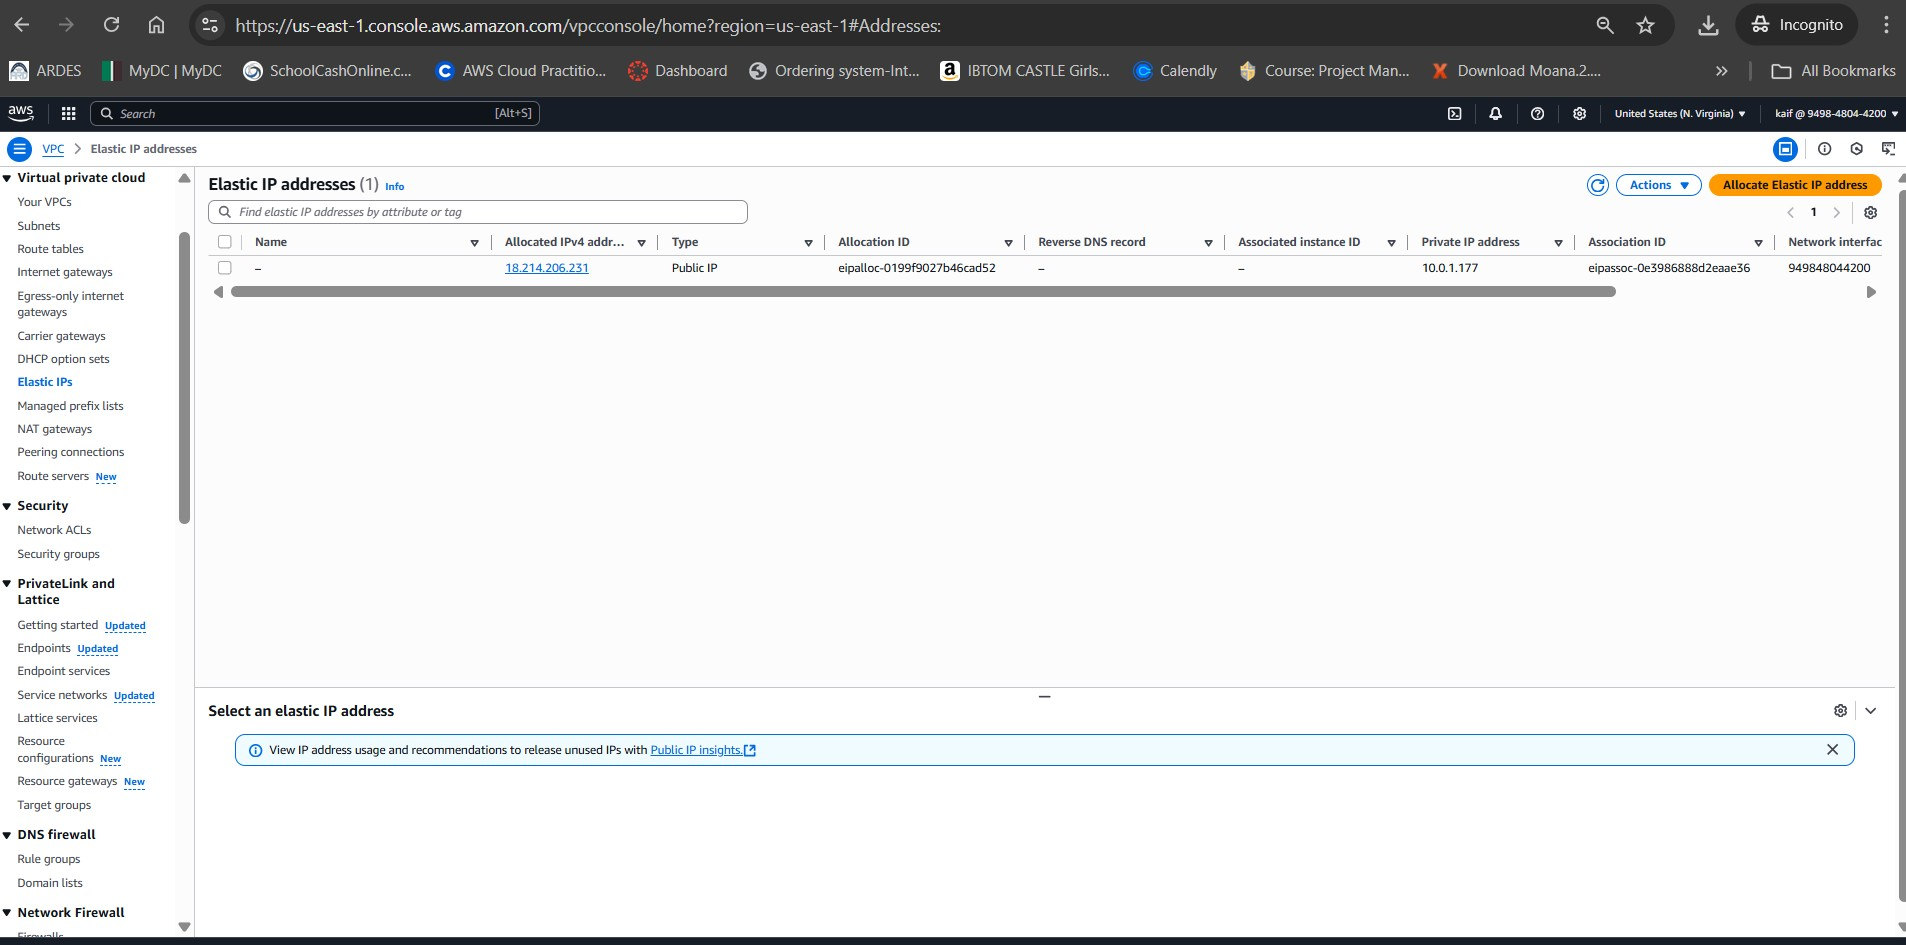
\includegraphics[width=0.8\textwidth]{elastic IP.jpg}
    \caption{Elastic IP assigned to the NAT Gateway.}
\end{figure}

\subsection{CI/CD Workflow and Final Documents}
\begin{figure}[h]
    \centering
    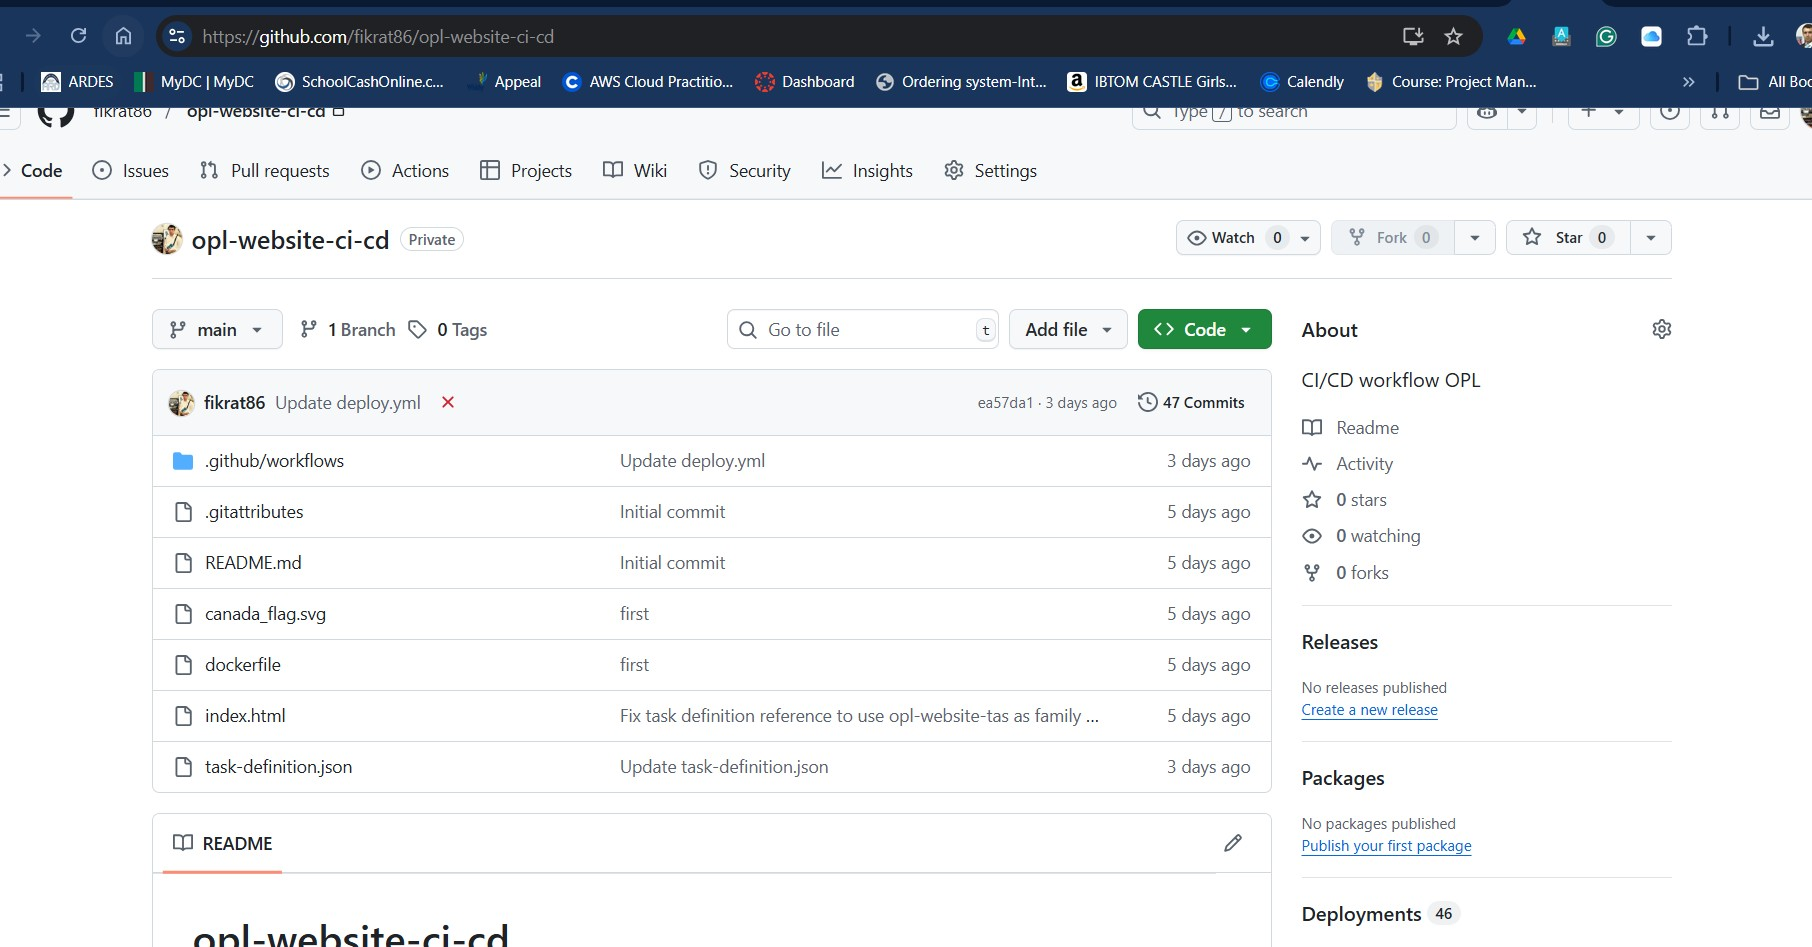
\includegraphics[width=0.8\textwidth]{github-repo.jpg}
    \caption{The GitHub repository containing the project files.}
\end{figure>
\begin{figure}[h]
    \centering
    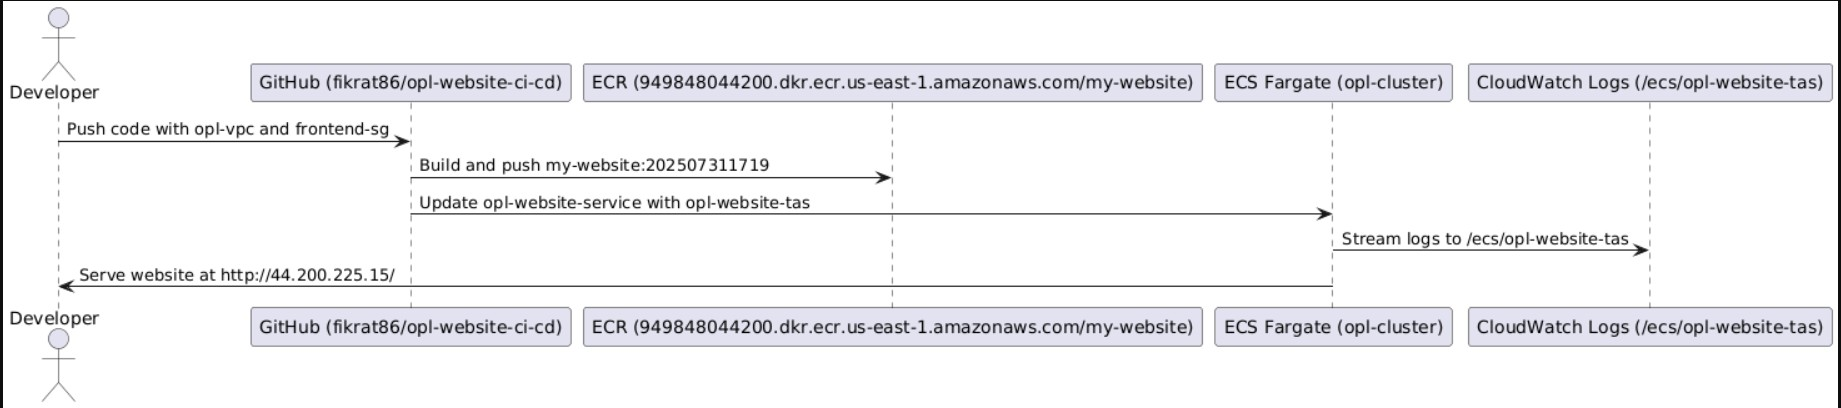
\includegraphics[width=0.8\textwidth]{CI_CD.jpg}
    \caption{The CI/CD workflow outline.}
\end{figure>
\begin{figure}[h]
    \centering
    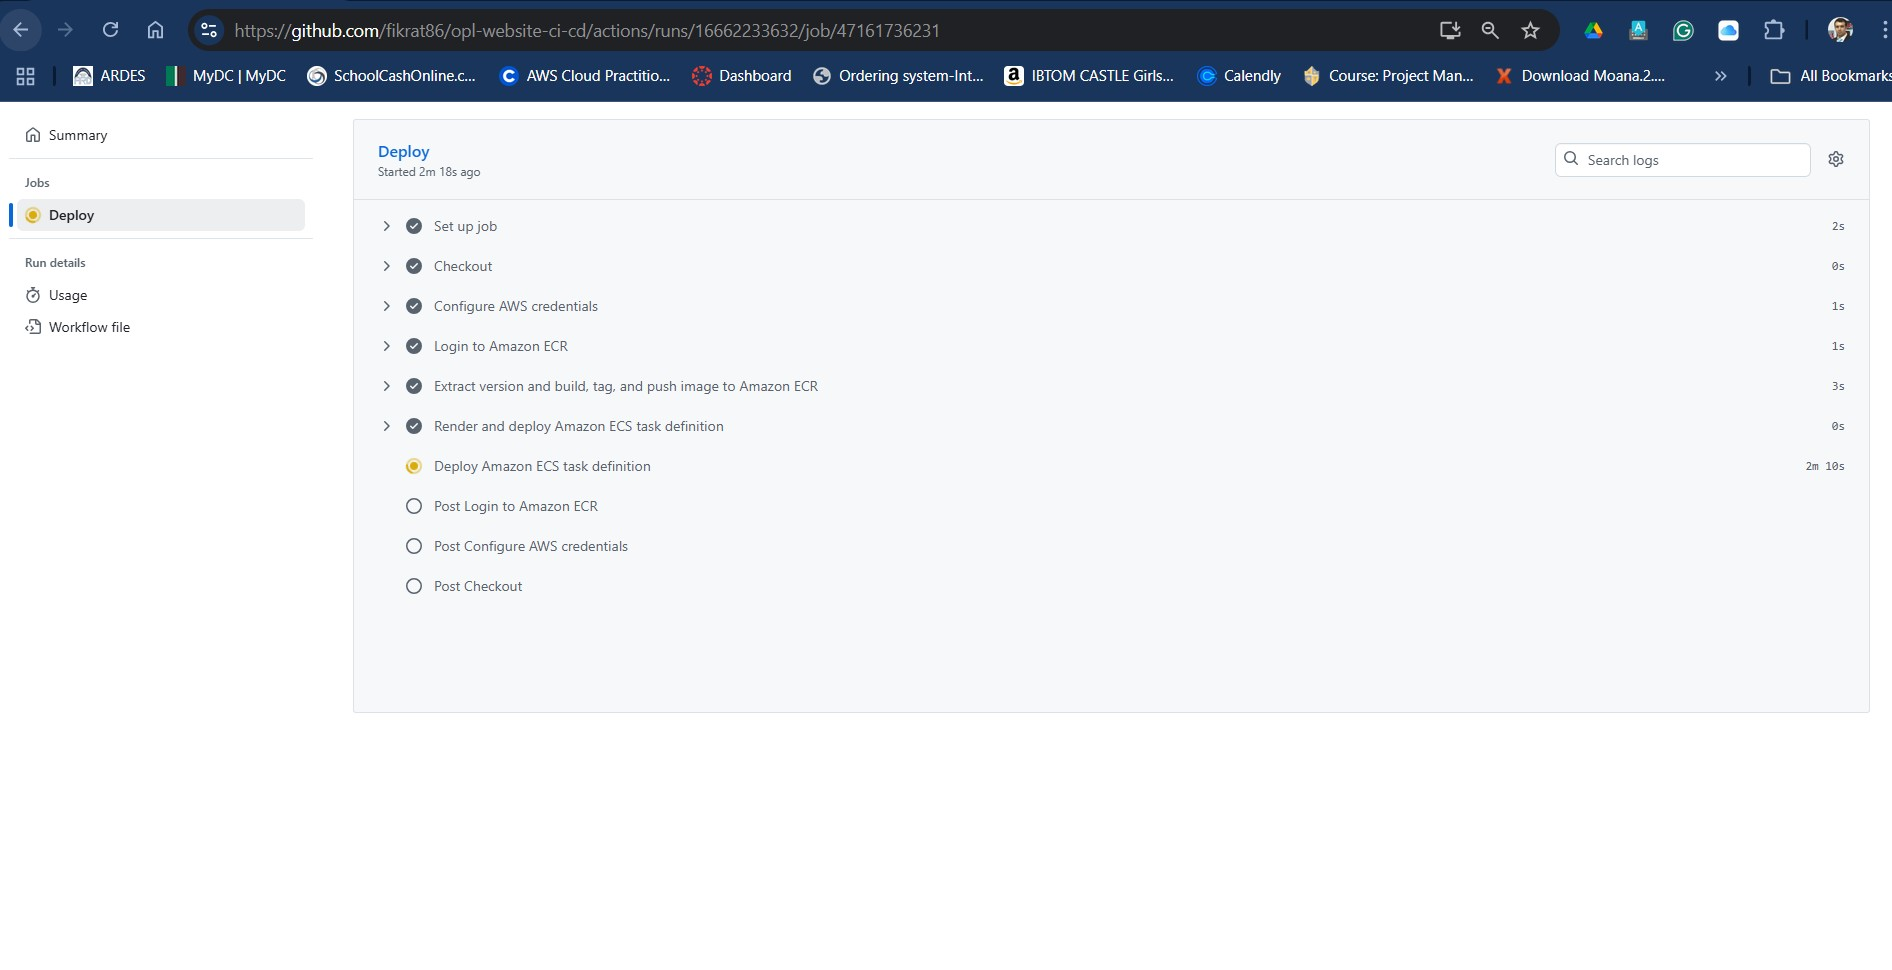
\includegraphics[width=0.8\textwidth]{deploy-workflow.jpg}
    \caption{The deployment workflow using GitHub Actions.}
\end{figure>
\begin{figure}[h]
    \centering
    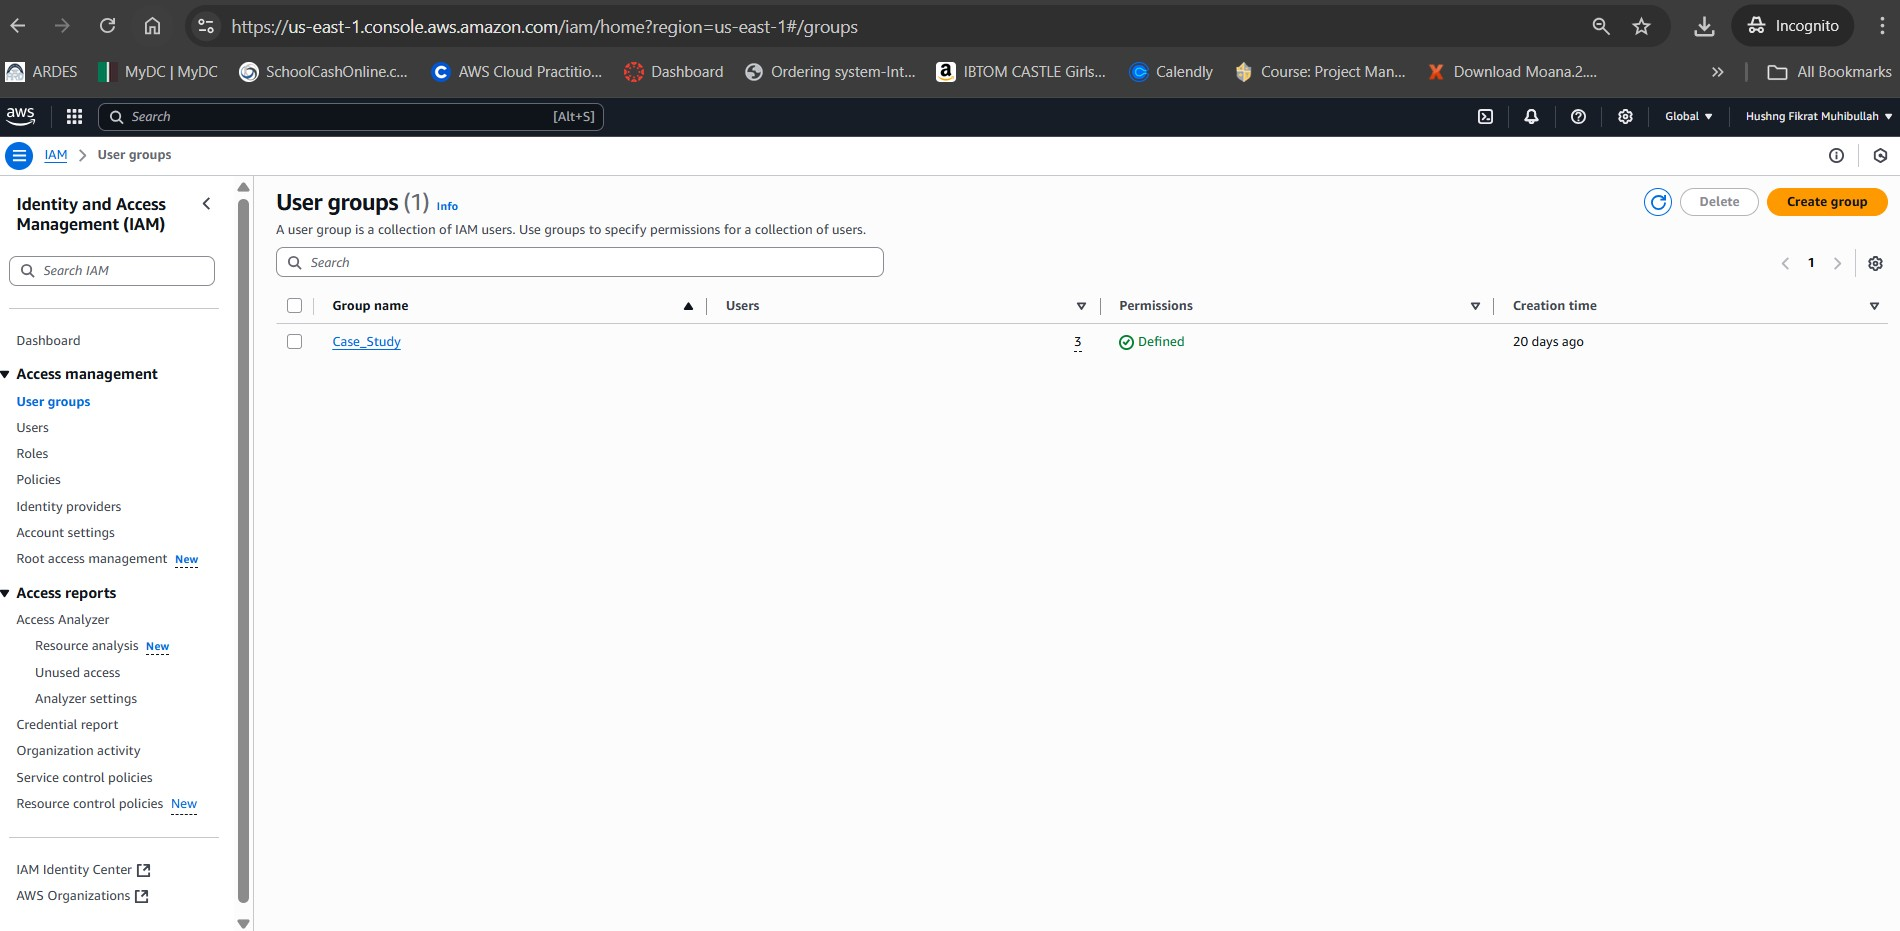
\includegraphics[width=0.8\textwidth]{group.jpg}
    \caption{Final team review and collaboration.}
\end{figure}

\section{Conclusion}
This case study comprehensively documents the CI/CD pipeline implementation for the OPL website using AWS ECS, supported by screenshots as proof of execution. The project successfully integrated Docker containerization, AWS networking, automated deployments, and robust monitoring, with each team member’s contributions validated. The solution is now production-ready, with all deployment, testing, and troubleshooting phases completed.

\end{document};